\documentclass[10pt, letterpaper, oneside, titlepage, landscape]{scrreprt}
% font size could be 10pt (default), 11pt or 12 pt
% paper size could be letterpaper (default), legalpaper, executivepaper,
% a4paper, a5paper or b5paper
% side could be oneside (default) or twoside
% columns could be onecolumn (default) or twocolumn
% graphics could be final (default) or draft
%
% titlepage could be notitlepage (default) or titlepage which
% makes an extra page for title
%
% paper alignment could be portrait (default) or landscape
%
% equations could be
%   default number of the equation on the right and equation centered
%   leqno number on the left and equation centered
%   fleqn number on the rigth and  equation on the left side
%

\usepackage{graphicx}
\usepackage{float}
\usepackage{color}
\usepackage{siunitx}
\usepackage[T1]{fontenc}
\usepackage{lmodern}
\usepackage{adjustbox}
\usepackage{array}
\usepackage{minitoc}
\usepackage{booktabs}
\usepackage{hyperref}
\hypersetup{
    colorlinks,
    citecolor=black,
    filecolor=black,
    linkcolor=black,
    urlcolor=black
}

\newcolumntype{R}[2]{%
    >{\adjustbox{angle=#1,lap=\width-(#2)}\bgroup}%
    l%
    <{\egroup}%
}

\usepackage{etoolbox}
\makeatletter
\patchcmd{\chapter}{\if@openright\cleardoublepage\else\clearpage\fi}{}{}{}
\makeatother

\newcommand*\rot{\multicolumn{1}{R{45}{1em}}}% no optional argument here, please
\title{$\Delta\Delta G$ Report --- zemu-values}
\subtitle{zemu-values ZEMu author values (ZEMu)}
\date{\today}
\begin{document}
\maketitle
\tableofcontents

\clearpage

\begin{abstract}
Prediction set scoring credit: ZEMu authors

\end{abstract}


\clearpage

\section{Data tables}

The predicted DDG value per case is computed using the 1 lowest-scoring mutant structures and the 1 lowest-scoring wildtype structures.

Derived mutations in analysis are omitted):

The stability classification cutoffs are: Experimental=1.00 kcal/mol, Predicted=1.00 energy units.
\subsection{Breakdown by volume}
\textit{A case is considered a small-to-large (resp. large-to-small) mutation if all of the wildtype residues have a smaller (resp. larger) van der Waals volume than the corresponding mutant residue. The order is defined as G < A < S < C < P < D < T < N < V < E < Q < H < ILM < FK < Y < R < W so some cases are considered to have no change in volume e.g. MET $\rightarrow$\ LEU.}

Not enough data for analysis of mutations no change in volume (at least 8 cases are required).


\begin{table}[H]\begin{center}
\begin{tabular}{ l S[table-format=3.2] l}
Statistic name & {Value} & p-value\\
\hline
Fraction correct & 0.65 & \\
Fraction correct (fuzzy) & 0.67 & \\
Gamma correlation coef. & 0.17 & \\
Kolmogorov-Smirnov test (XY) & 0.18 & (2-tailed p-value=$2.57\times10^{-01}$)\\
MAE & 1.09 & \\
Pearson's R & 0.48 & (2-tailed p-value=$8.65\times10^{-05}$)\\
Spearman's R & 0.24 & (2-tailed p-value=$6.45\times10^{-02}$)\\
X-axis Kolmogorov-Smirnov test & 0.13 & (p-value=$2.29\times10^{-01}$)\\
X-axis normality test & 2.18 & (2-sided chi$^{2}$ p-value=$3.36\times10^{-01}$)\\
Y-axis Kolmogorov-Smirnov test & 0.15 & (p-value=$1.07\times10^{-01}$)\\
Y-axis normality test & 59.66 & (2-sided chi$^{2}$ p-value=$1.11\times10^{-13}$)\\
n & 62.00 & \\
num\_null\_cases & 0.00 & \\
\end{tabular}
\caption{Statistics - small-to-large mutations (62 cases)}
\end{center}\end{table}




\begin{table}[H]\begin{center}
\begin{tabular}{ l S[table-format=3.2] l}
Statistic name & {Value} & p-value\\
\hline
Fraction correct & 0.71 & \\
Fraction correct (fuzzy) & 0.72 & \\
Gamma correlation coef. & 0.37 & \\
Kolmogorov-Smirnov test (XY) & 0.18 & (2-tailed p-value=$1.37\times10^{-07}$)\\
MAE & 1.08 & \\
Pearson's R & 0.57 & (2-tailed p-value=$4.53\times10^{-43}$)\\
Spearman's R & 0.53 & (2-tailed p-value=$2.06\times10^{-37}$)\\
X-axis Kolmogorov-Smirnov test & 0.36 & (p-value=$0.00\times10^{+00}$)\\
X-axis normality test & 92.92 & (2-sided chi$^{2}$ p-value=$6.64\times10^{-21}$)\\
Y-axis Kolmogorov-Smirnov test & 0.25 & (p-value=$0.00\times10^{+00}$)\\
Y-axis normality test & 153.78 & (2-sided chi$^{2}$ p-value=$4.04\times10^{-34}$)\\
n & 488.00 & \\
num\_null\_cases & 0.00 & \\
\end{tabular}
\caption{Statistics - large-to-small mutations (488 cases)}
\end{center}\end{table}


\subsection{Separating out mutations involving glycine or proline.}
\textit{This cases may involve changes to secondary structure so we separate them out here.}



\begin{table}[H]\begin{center}
\begin{tabular}{ l S[table-format=3.2] l}
Statistic name & {Value} & p-value\\
\hline
Fraction correct & 0.65 & \\
Fraction correct (fuzzy) & 0.64 & \\
Gamma correlation coef. & 0.55 & \\
Kolmogorov-Smirnov test (XY) & 0.24 & (2-tailed p-value=$2.65\times10^{-01}$)\\
MAE & 1.55 & \\
Pearson's R & 0.69 & (2-tailed p-value=$5.16\times10^{-06}$)\\
Spearman's R & 0.73 & (2-tailed p-value=$8.11\times10^{-07}$)\\
X-axis Kolmogorov-Smirnov test & 0.52 & (p-value=$4.57\times10^{-09}$)\\
X-axis normality test & 0.66 & (2-sided chi$^{2}$ p-value=$7.21\times10^{-01}$)\\
Y-axis Kolmogorov-Smirnov test & 0.34 & (p-value=$4.31\times10^{-04}$)\\
Y-axis normality test & 14.61 & (2-sided chi$^{2}$ p-value=$6.72\times10^{-04}$)\\
n & 34.00 & \\
num\_null\_cases & 0.00 & \\
\end{tabular}
\caption{Statistics - cases with G or P (34 cases)}
\end{center}\end{table}




\begin{table}[H]\begin{center}
\begin{tabular}{ l S[table-format=3.2] l}
Statistic name & {Value} & p-value\\
\hline
Fraction correct & 0.71 & \\
Fraction correct (fuzzy) & 0.72 & \\
Gamma correlation coef. & 0.37 & \\
Kolmogorov-Smirnov test (XY) & 0.17 & (2-tailed p-value=$1.35\times10^{-07}$)\\
MAE & 1.07 & \\
Pearson's R & 0.56 & (2-tailed p-value=$9.10\times10^{-45}$)\\
Spearman's R & 0.53 & (2-tailed p-value=$3.70\times10^{-39}$)\\
X-axis Kolmogorov-Smirnov test & 0.31 & (p-value=$0.00\times10^{+00}$)\\
X-axis normality test & 57.49 & (2-sided chi$^{2}$ p-value=$3.28\times10^{-13}$)\\
Y-axis Kolmogorov-Smirnov test & 0.22 & (p-value=$0.00\times10^{+00}$)\\
Y-axis normality test & 171.27 & (2-sided chi$^{2}$ p-value=$6.46\times10^{-38}$)\\
n & 532.00 & \\
num\_null\_cases & 0.00 & \\
\end{tabular}
\caption{Statistics - cases without G or P (532 cases)}
\end{center}\end{table}


\subsection{Number of mutations}



\begin{table}[H]\begin{center}
\begin{tabular}{ l S[table-format=3.2] l}
Statistic name & {Value} & p-value\\
\hline
Fraction correct & 0.69 & \\
Fraction correct (fuzzy) & 0.70 & \\
Gamma correlation coef. & 0.30 & \\
Kolmogorov-Smirnov test (XY) & 0.19 & (2-tailed p-value=$8.34\times10^{-08}$)\\
MAE & 0.99 & \\
Pearson's R & 0.54 & (2-tailed p-value=$3.07\times10^{-35}$)\\
Spearman's R & 0.44 & (2-tailed p-value=$5.54\times10^{-23}$)\\
X-axis Kolmogorov-Smirnov test & 0.32 & (p-value=$0.00\times10^{+00}$)\\
X-axis normality test & 116.40 & (2-sided chi$^{2}$ p-value=$5.29\times10^{-26}$)\\
Y-axis Kolmogorov-Smirnov test & 0.23 & (p-value=$0.00\times10^{+00}$)\\
Y-axis normality test & 169.06 & (2-sided chi$^{2}$ p-value=$1.95\times10^{-37}$)\\
n & 453.00 & \\
num\_null\_cases & 0.00 & \\
\end{tabular}
\caption{Statistics - single mutations (453 cases)}
\end{center}\end{table}




\begin{table}[H]\begin{center}
\begin{tabular}{ l S[table-format=3.2] l}
Statistic name & {Value} & p-value\\
\hline
Fraction correct & 0.76 & \\
Fraction correct (fuzzy) & 0.77 & \\
Gamma correlation coef. & 0.50 & \\
Kolmogorov-Smirnov test (XY) & 0.11 & (2-tailed p-value=$5.24\times10^{-01}$)\\
MAE & 1.56 & \\
Pearson's R & 0.62 & (2-tailed p-value=$1.66\times10^{-13}$)\\
Spearman's R & 0.70 & (2-tailed p-value=$7.66\times10^{-18}$)\\
X-axis Kolmogorov-Smirnov test & 0.45 & (p-value=$0.00\times10^{+00}$)\\
X-axis normality test & 4.54 & (2-sided chi$^{2}$ p-value=$1.03\times10^{-01}$)\\
Y-axis Kolmogorov-Smirnov test & 0.41 & (p-value=$0.00\times10^{+00}$)\\
Y-axis normality test & 11.63 & (2-sided chi$^{2}$ p-value=$2.99\times10^{-03}$)\\
n & 113.00 & \\
num\_null\_cases & 0.00 & \\
\end{tabular}
\caption{Statistics - multiple mutations (113 cases)}
\end{center}\end{table}


\subsection{Entire dataset using a scaling factor of 1/1.274 to improve the fraction correct metric.}
\textit{Warning: Results in this section use an averaged scaling factor to improve the value for the fraction correct metric. This scalar will vary over benchmark runs so these results should not be interpreted as performance results; they should be considered as what could be obtained if the predicted values were scaled by a "magic" value.}



\begin{table}[H]\begin{center}
\begin{tabular}{ l S[table-format=3.2] l}
Statistic name & {Value} & p-value\\
\hline
Fraction correct & 0.71 & \\
Fraction correct (fuzzy) & 0.72 & \\
Gamma correlation coef. & 0.38 & \\
Kolmogorov-Smirnov test (XY) & 0.19 & (2-tailed p-value=$5.17\times10^{-09}$)\\
MAE & 1.03 & \\
Pearson's R & 0.58 & (2-tailed p-value=$6.86\times10^{-52}$)\\
Spearman's R & 0.55 & (2-tailed p-value=$2.69\times10^{-45}$)\\
X-axis Kolmogorov-Smirnov test & 0.31 & (p-value=$0.00\times10^{+00}$)\\
X-axis normality test & 52.55 & (2-sided chi$^{2}$ p-value=$3.88\times10^{-12}$)\\
Y-axis Kolmogorov-Smirnov test & 0.25 & (p-value=$0.00\times10^{+00}$)\\
Y-axis normality test & 191.99 & (2-sided chi$^{2}$ p-value=$2.04\times10^{-42}$)\\
n & 566.00 & \\
num\_null\_cases & 0.00 & \\
\end{tabular}
\caption{Statistics - complete dataset (scaled) (566 cases)}
\end{center}\end{table}


\subsection{Entire dataset}
\textit{Overall statistics}



\begin{table}[H]\begin{center}
\begin{tabular}{ l S[table-format=3.2] l}
Statistic name & {Value} & p-value\\
\hline
Fraction correct & 0.70 & \\
Fraction correct (fuzzy) & 0.71 & \\
Gamma correlation coef. & 0.38 & \\
Kolmogorov-Smirnov test (XY) & 0.17 & (2-tailed p-value=$2.62\times10^{-07}$)\\
MAE & 1.10 & \\
Pearson's R & 0.58 & (2-tailed p-value=$6.86\times10^{-52}$)\\
Spearman's R & 0.55 & (2-tailed p-value=$2.69\times10^{-45}$)\\
X-axis Kolmogorov-Smirnov test & 0.31 & (p-value=$0.00\times10^{+00}$)\\
X-axis normality test & 52.55 & (2-sided chi$^{2}$ p-value=$3.88\times10^{-12}$)\\
Y-axis Kolmogorov-Smirnov test & 0.22 & (p-value=$0.00\times10^{+00}$)\\
Y-axis normality test & 191.99 & (2-sided chi$^{2}$ p-value=$2.04\times10^{-42}$)\\
n & 566.00 & \\
num\_null\_cases & 0.00 & \\
\end{tabular}
\caption{Statistics - complete dataset (566 cases)}
\end{center}\end{table}



\clearpage

\section{Main plots}

\begin{figure}[H]
  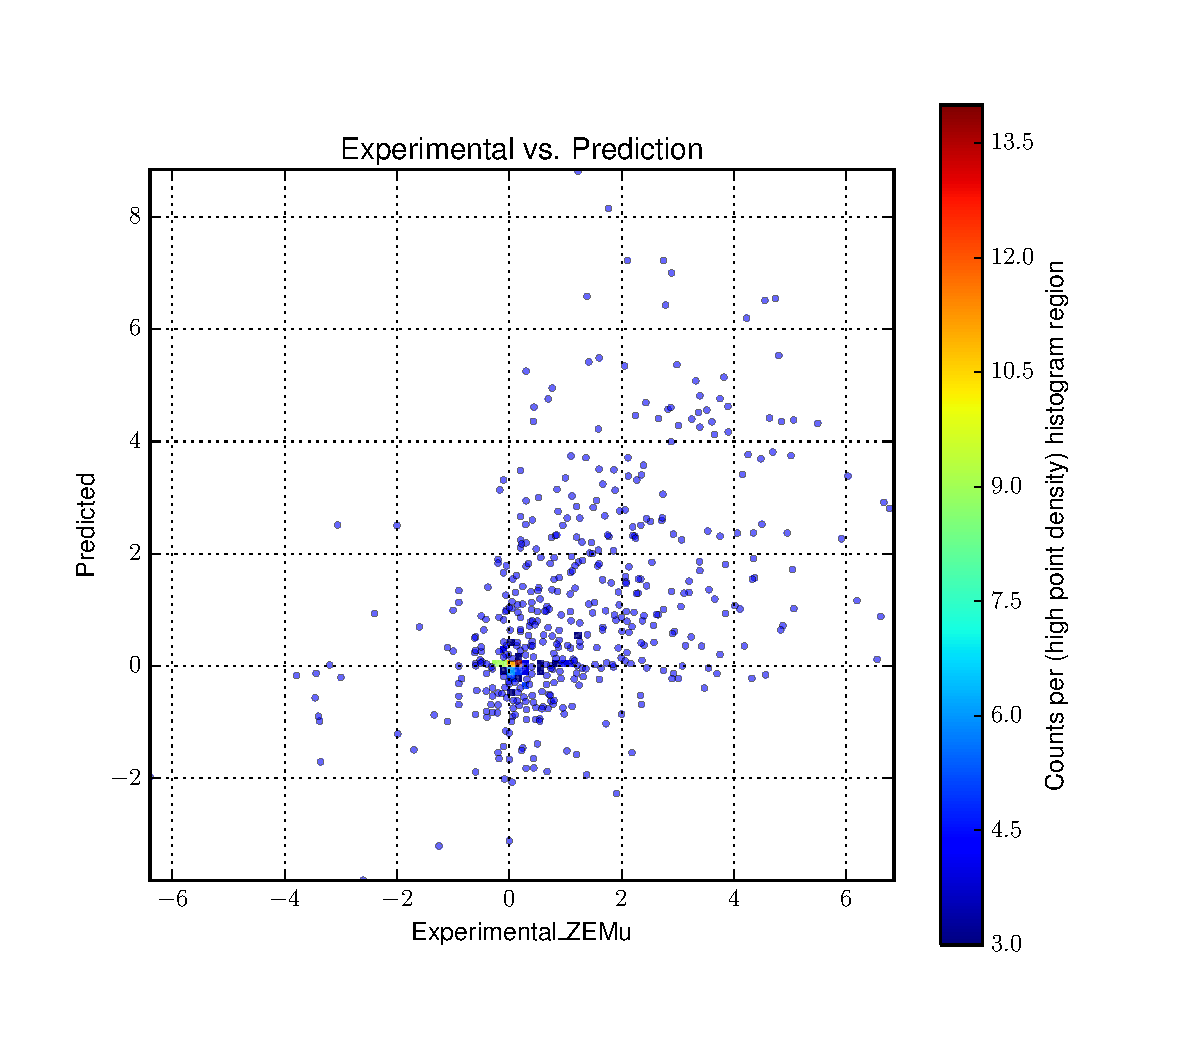
\includegraphics[width=\textwidth]{{/tmp/kyleb/multiple_analysis/analysis_sets/ZEMu/topx_1-prediction_set_id_zemu-values-score_method_zemu-paper/zemu-values_subplots/experimental_prediction_scatter}.pdf}
  \caption{Experimental vs. Predicted scatterplot (with density binning)}
\end{figure}
\begin{figure}[H]
  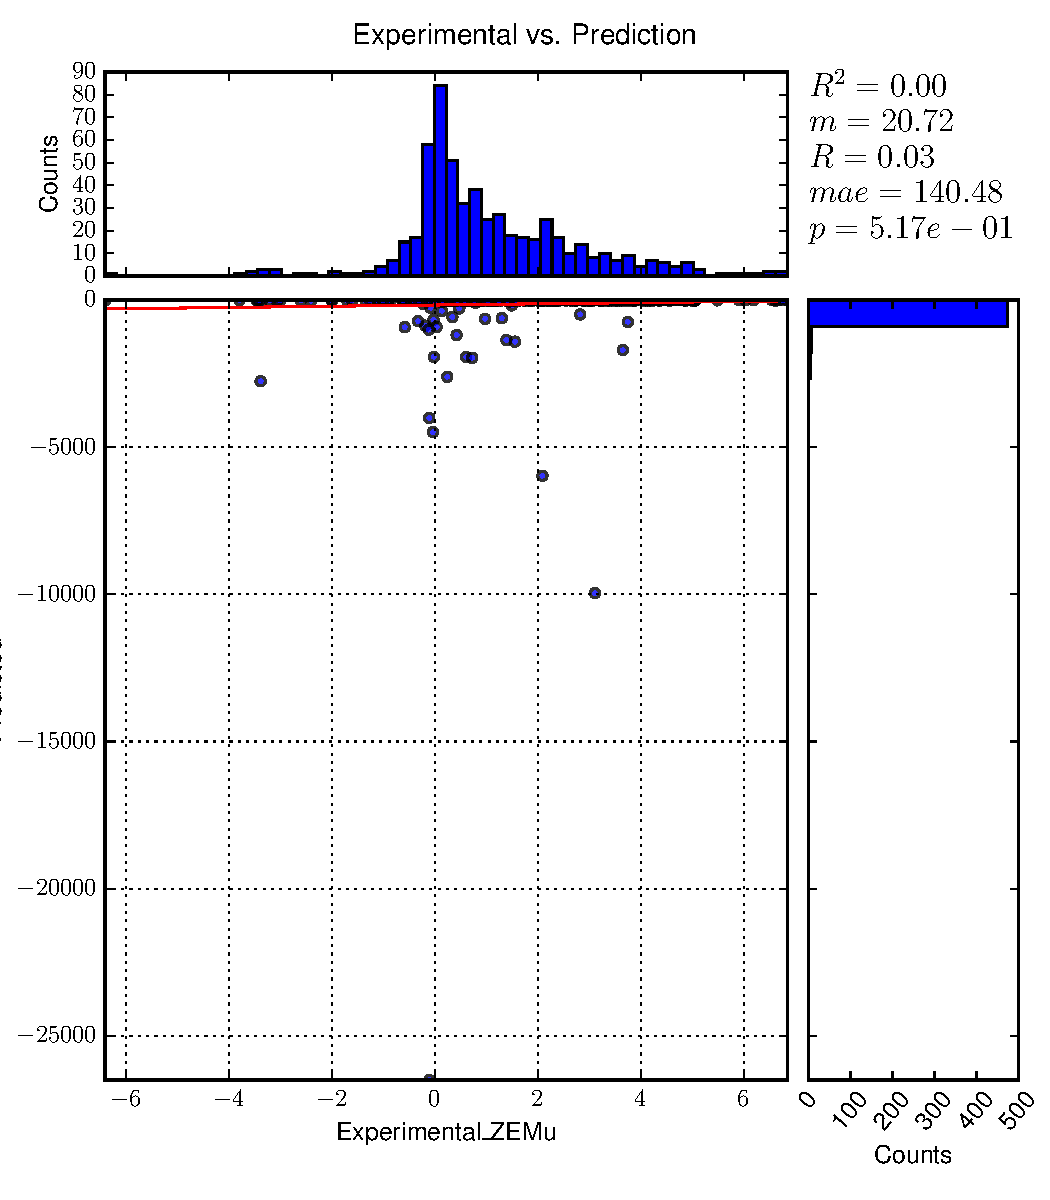
\includegraphics[width=\textwidth]{{/tmp/kyleb/multiple_analysis/analysis_sets/ZEMu/topx_1-prediction_set_id_zemu-values-score_method_zemu-paper/zemu-values_subplots/histogram_fit_scatter}.pdf}
  \caption{Experimental vs. Predicted scatterplot, with histograms and linear fit statistics. The p-value here (if present) indicates the likelihood that a random set of this many points would produce a correlation at least as strong as the observed correlation.}
\end{figure}
\begin{figure}[H]
  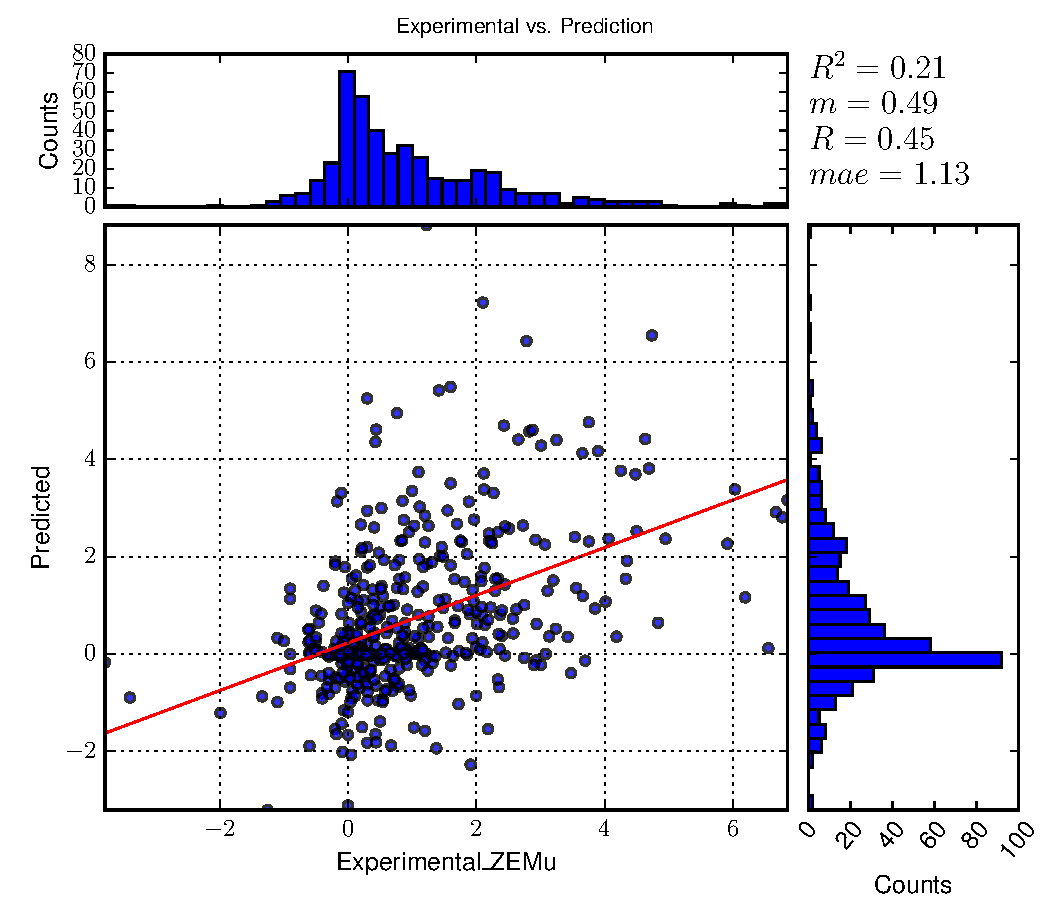
\includegraphics[width=\textwidth]{{/tmp/kyleb/multiple_analysis/analysis_sets/ZEMu/topx_1-prediction_set_id_zemu-values-score_method_zemu-paper/zemu-values_subplots/single_mutations_histogram_fit_scatter}.pdf}
  \caption{Single mutations data subset}
\end{figure}
\begin{figure}[H]
  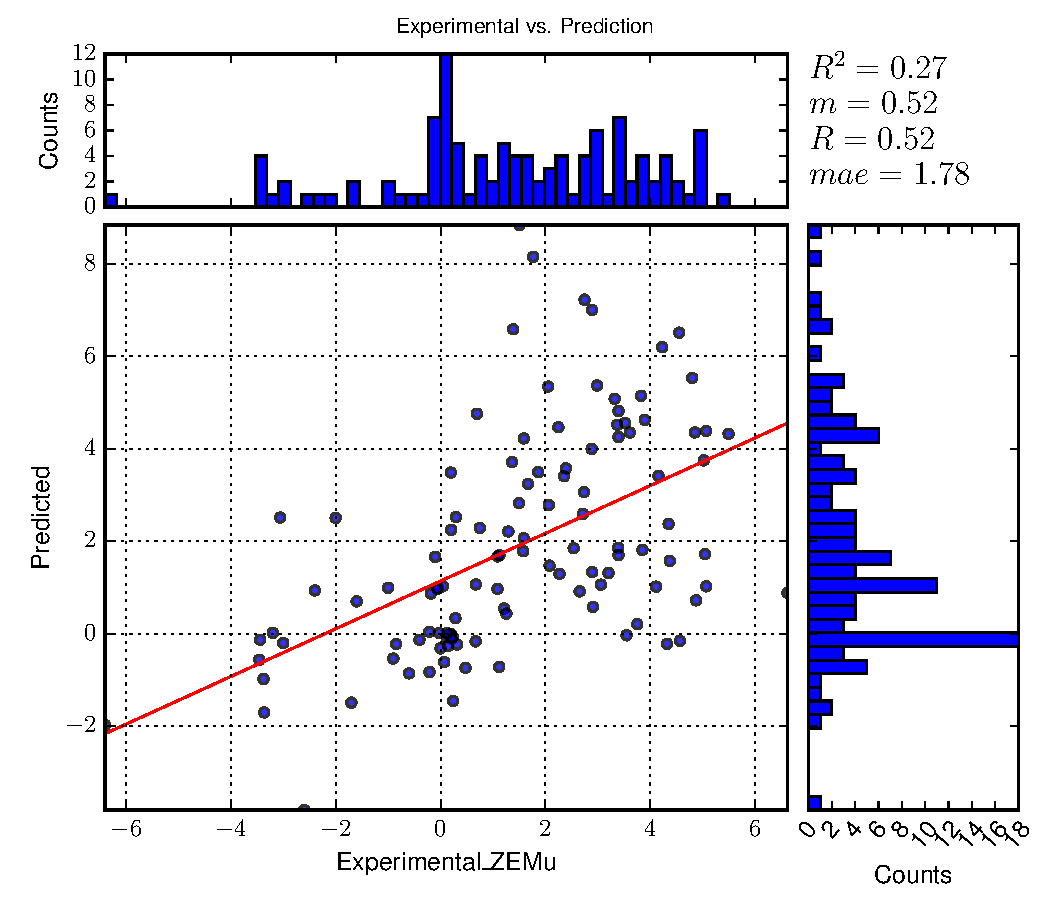
\includegraphics[width=\textwidth]{{/tmp/kyleb/multiple_analysis/analysis_sets/ZEMu/topx_1-prediction_set_id_zemu-values-score_method_zemu-paper/zemu-values_subplots/multiple_mutations_histogram_fit_scatter}.pdf}
  \caption{Multiple mutations data subset}
\end{figure}
\begin{figure}[H]
  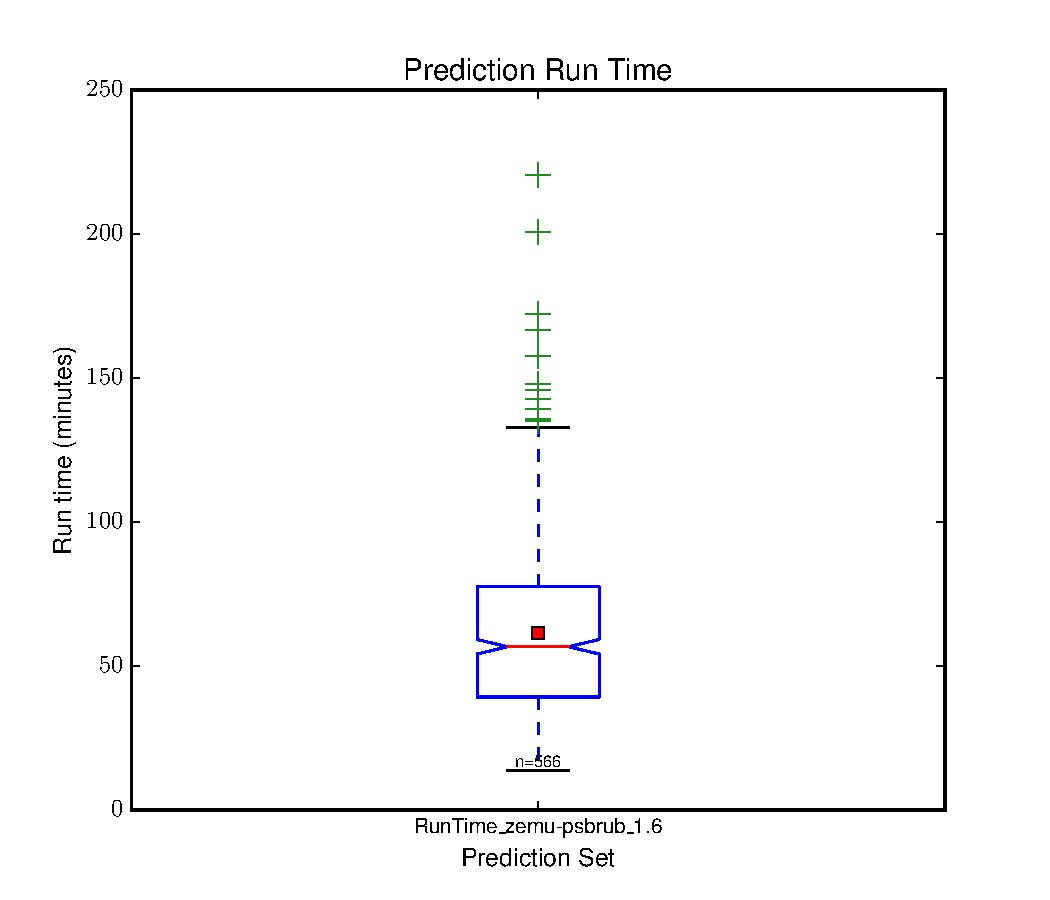
\includegraphics[width=\textwidth]{{/tmp/kyleb/multiple_analysis/analysis_sets/ZEMu/topx_1-prediction_set_id_zemu-values-score_method_zemu-paper/zemu-values_subplots/runtime}.pdf}
  \caption{Run time}
\end{figure}
\begin{figure}[H]
  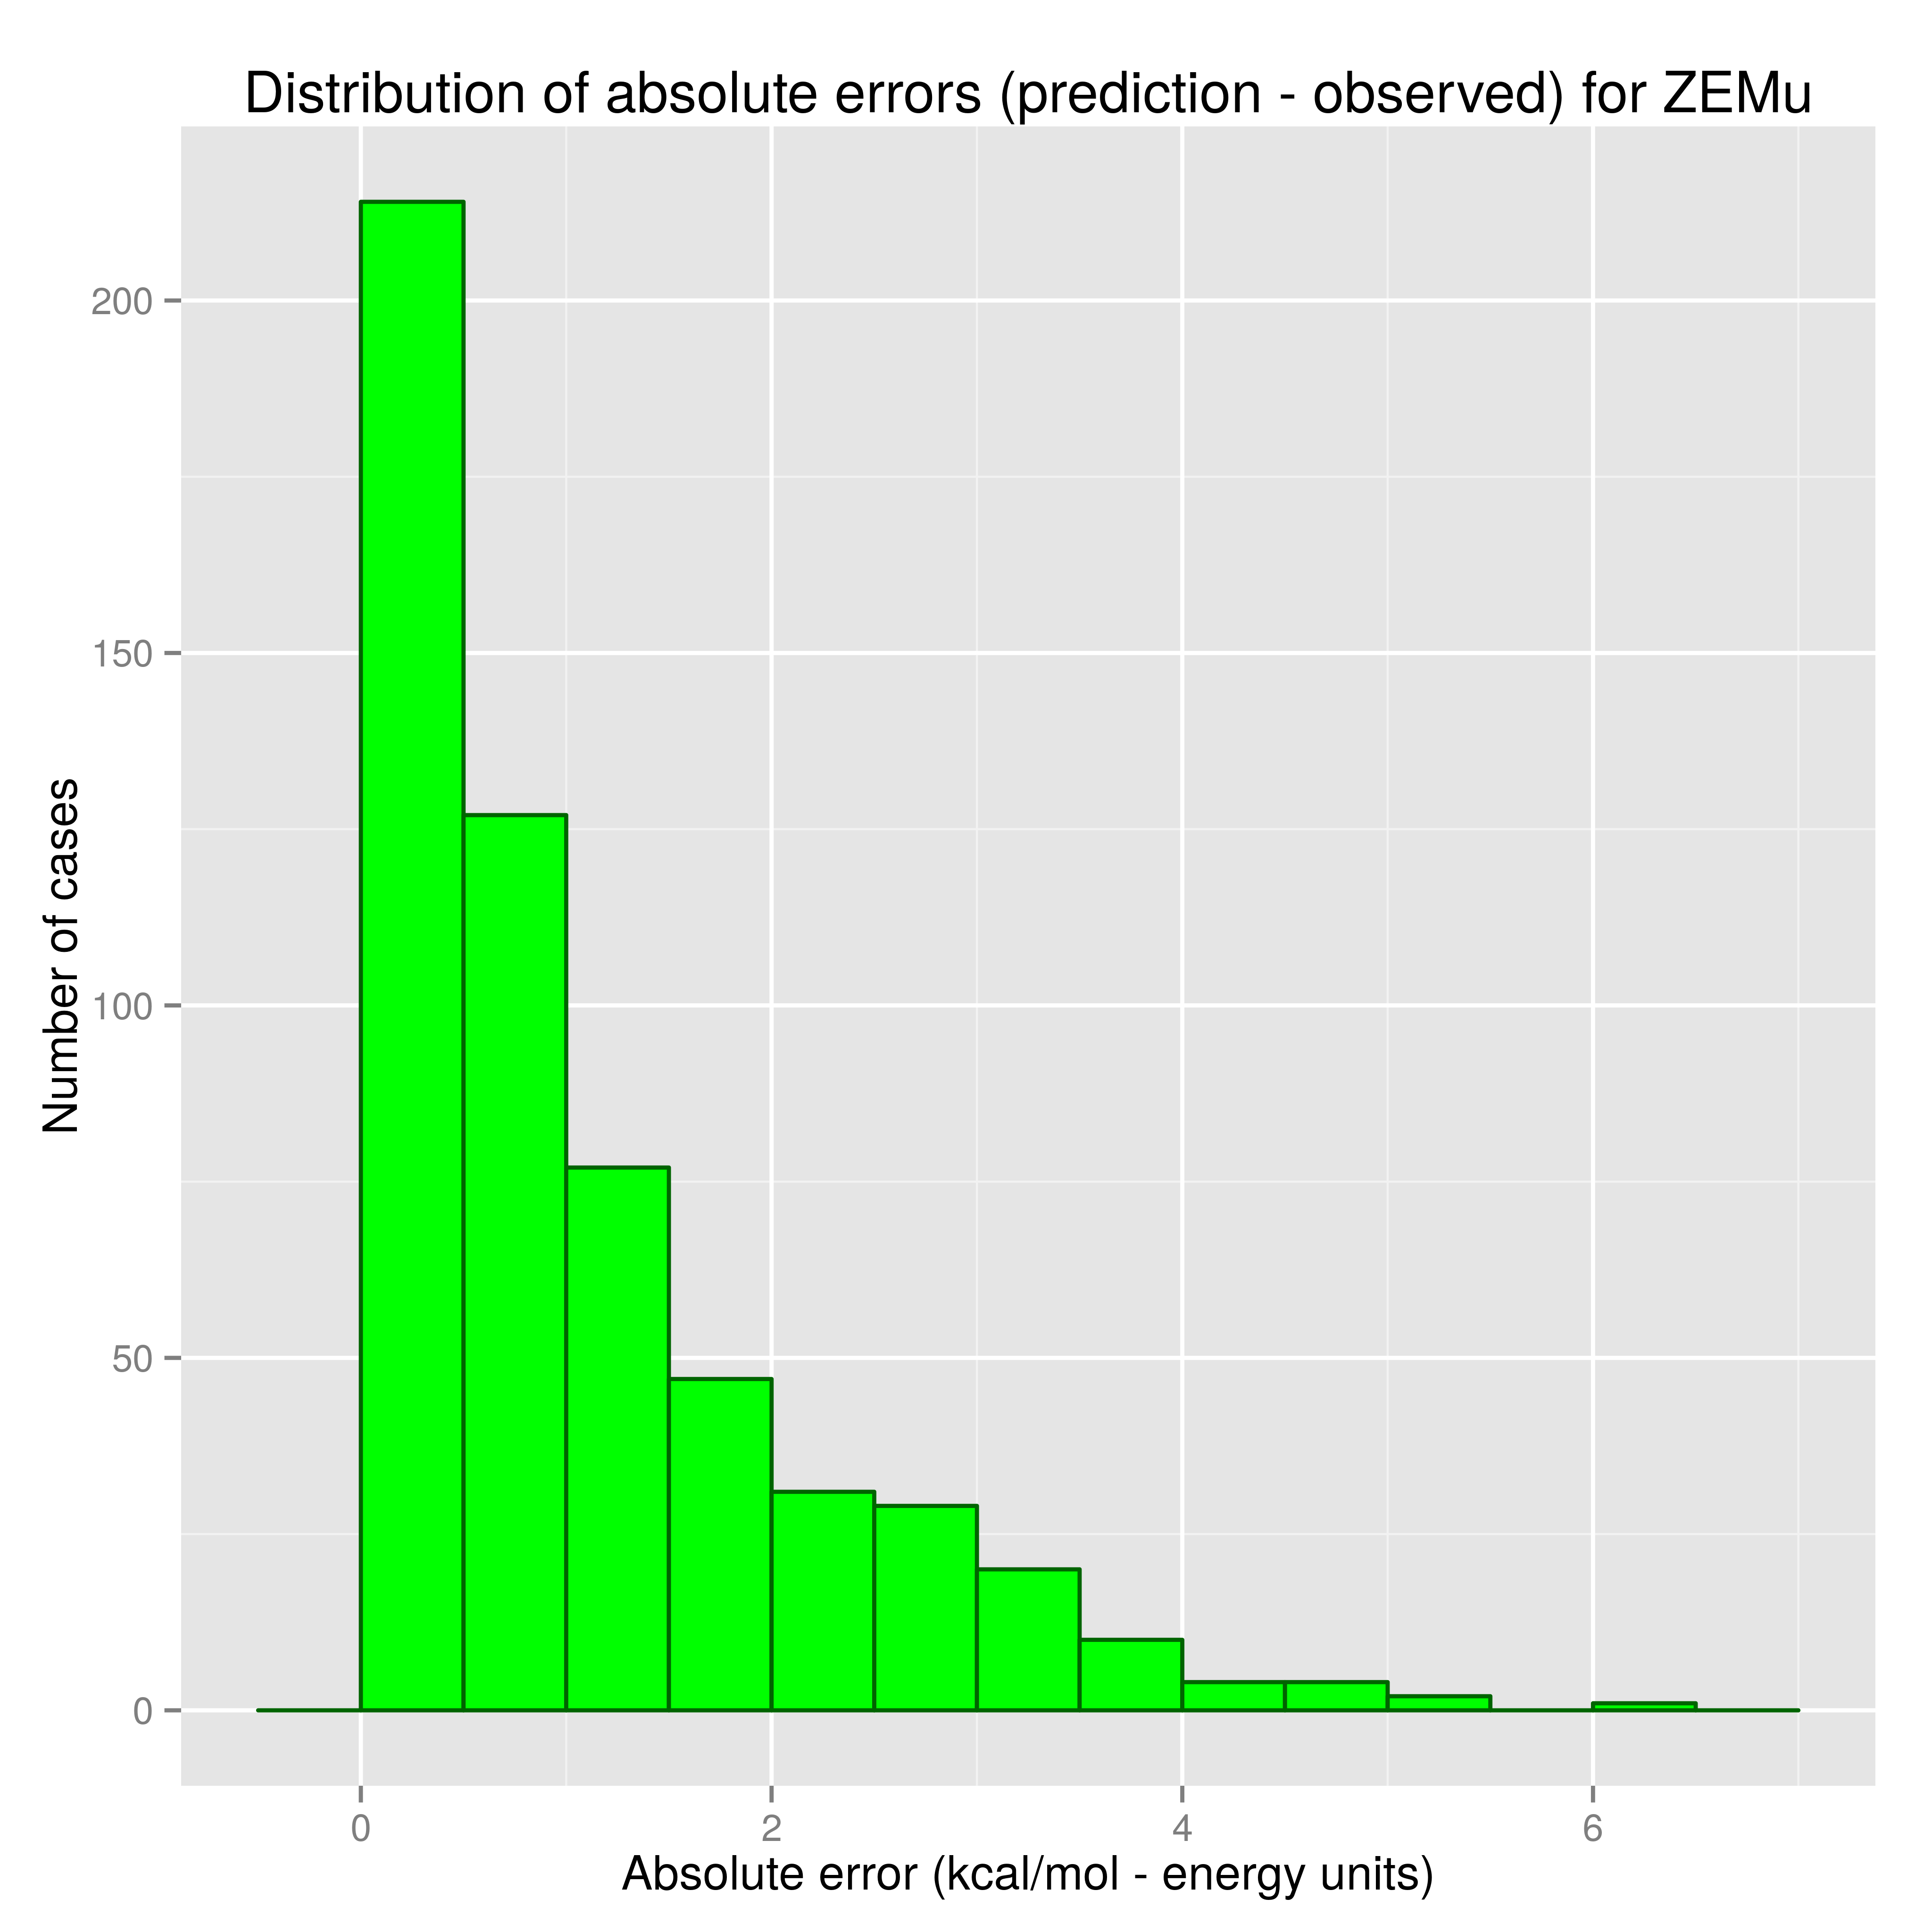
\includegraphics[width=\textwidth]{{/tmp/kyleb/multiple_analysis/analysis_sets/ZEMu/topx_1-prediction_set_id_zemu-values-score_method_zemu-paper/zemu-values_subplots/zemu-values_ZEMu_absolute_errors}.png}
  \caption{Absolute error histogram}
\end{figure}

\clearpage

\section{Adjustments}
\textit{Optimization of the cutoffs
for the fraction correct metric}

\begin{figure}[H]
  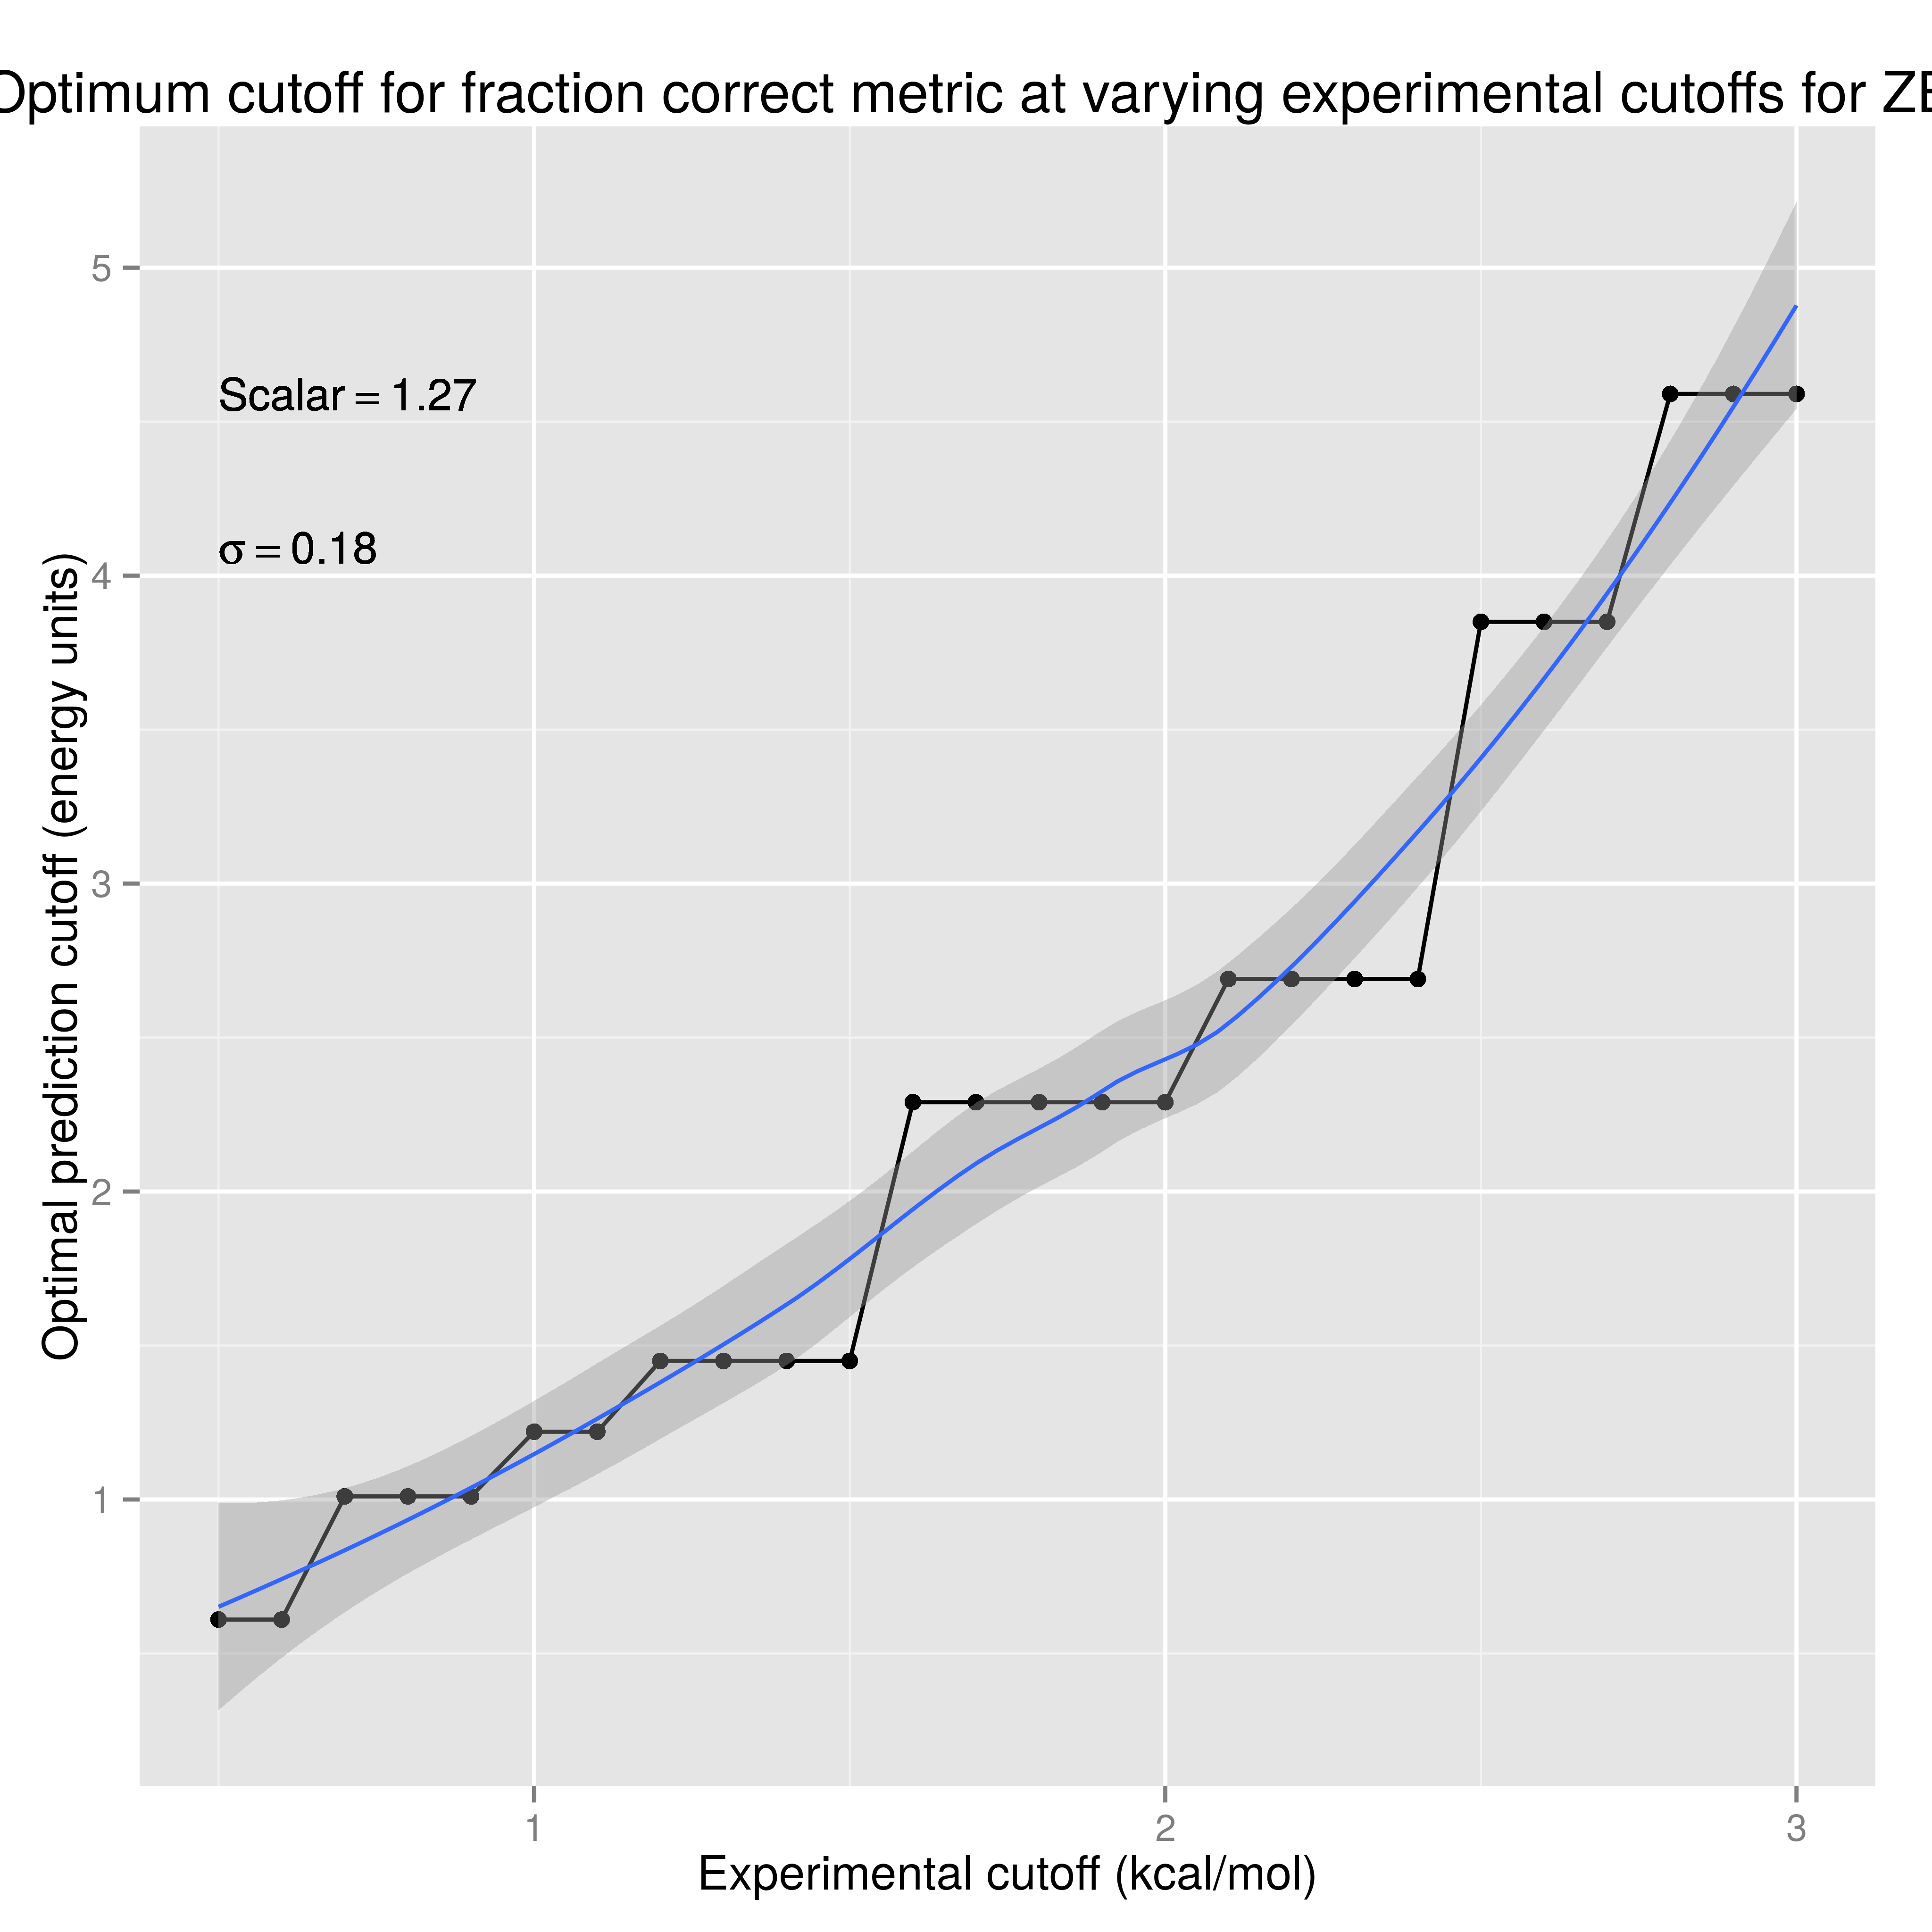
\includegraphics[width=\textwidth]{{/tmp/kyleb/multiple_analysis/analysis_sets/ZEMu/topx_1-prediction_set_id_zemu-values-score_method_zemu-paper/zemu-values_subplots/zemu-values_ZEMu_optimum_fraction_correct_at_varying_kcal_mol}.png}
  \caption{Scalar adjustment calculation plot}
\end{figure}
\begin{figure}[H]
  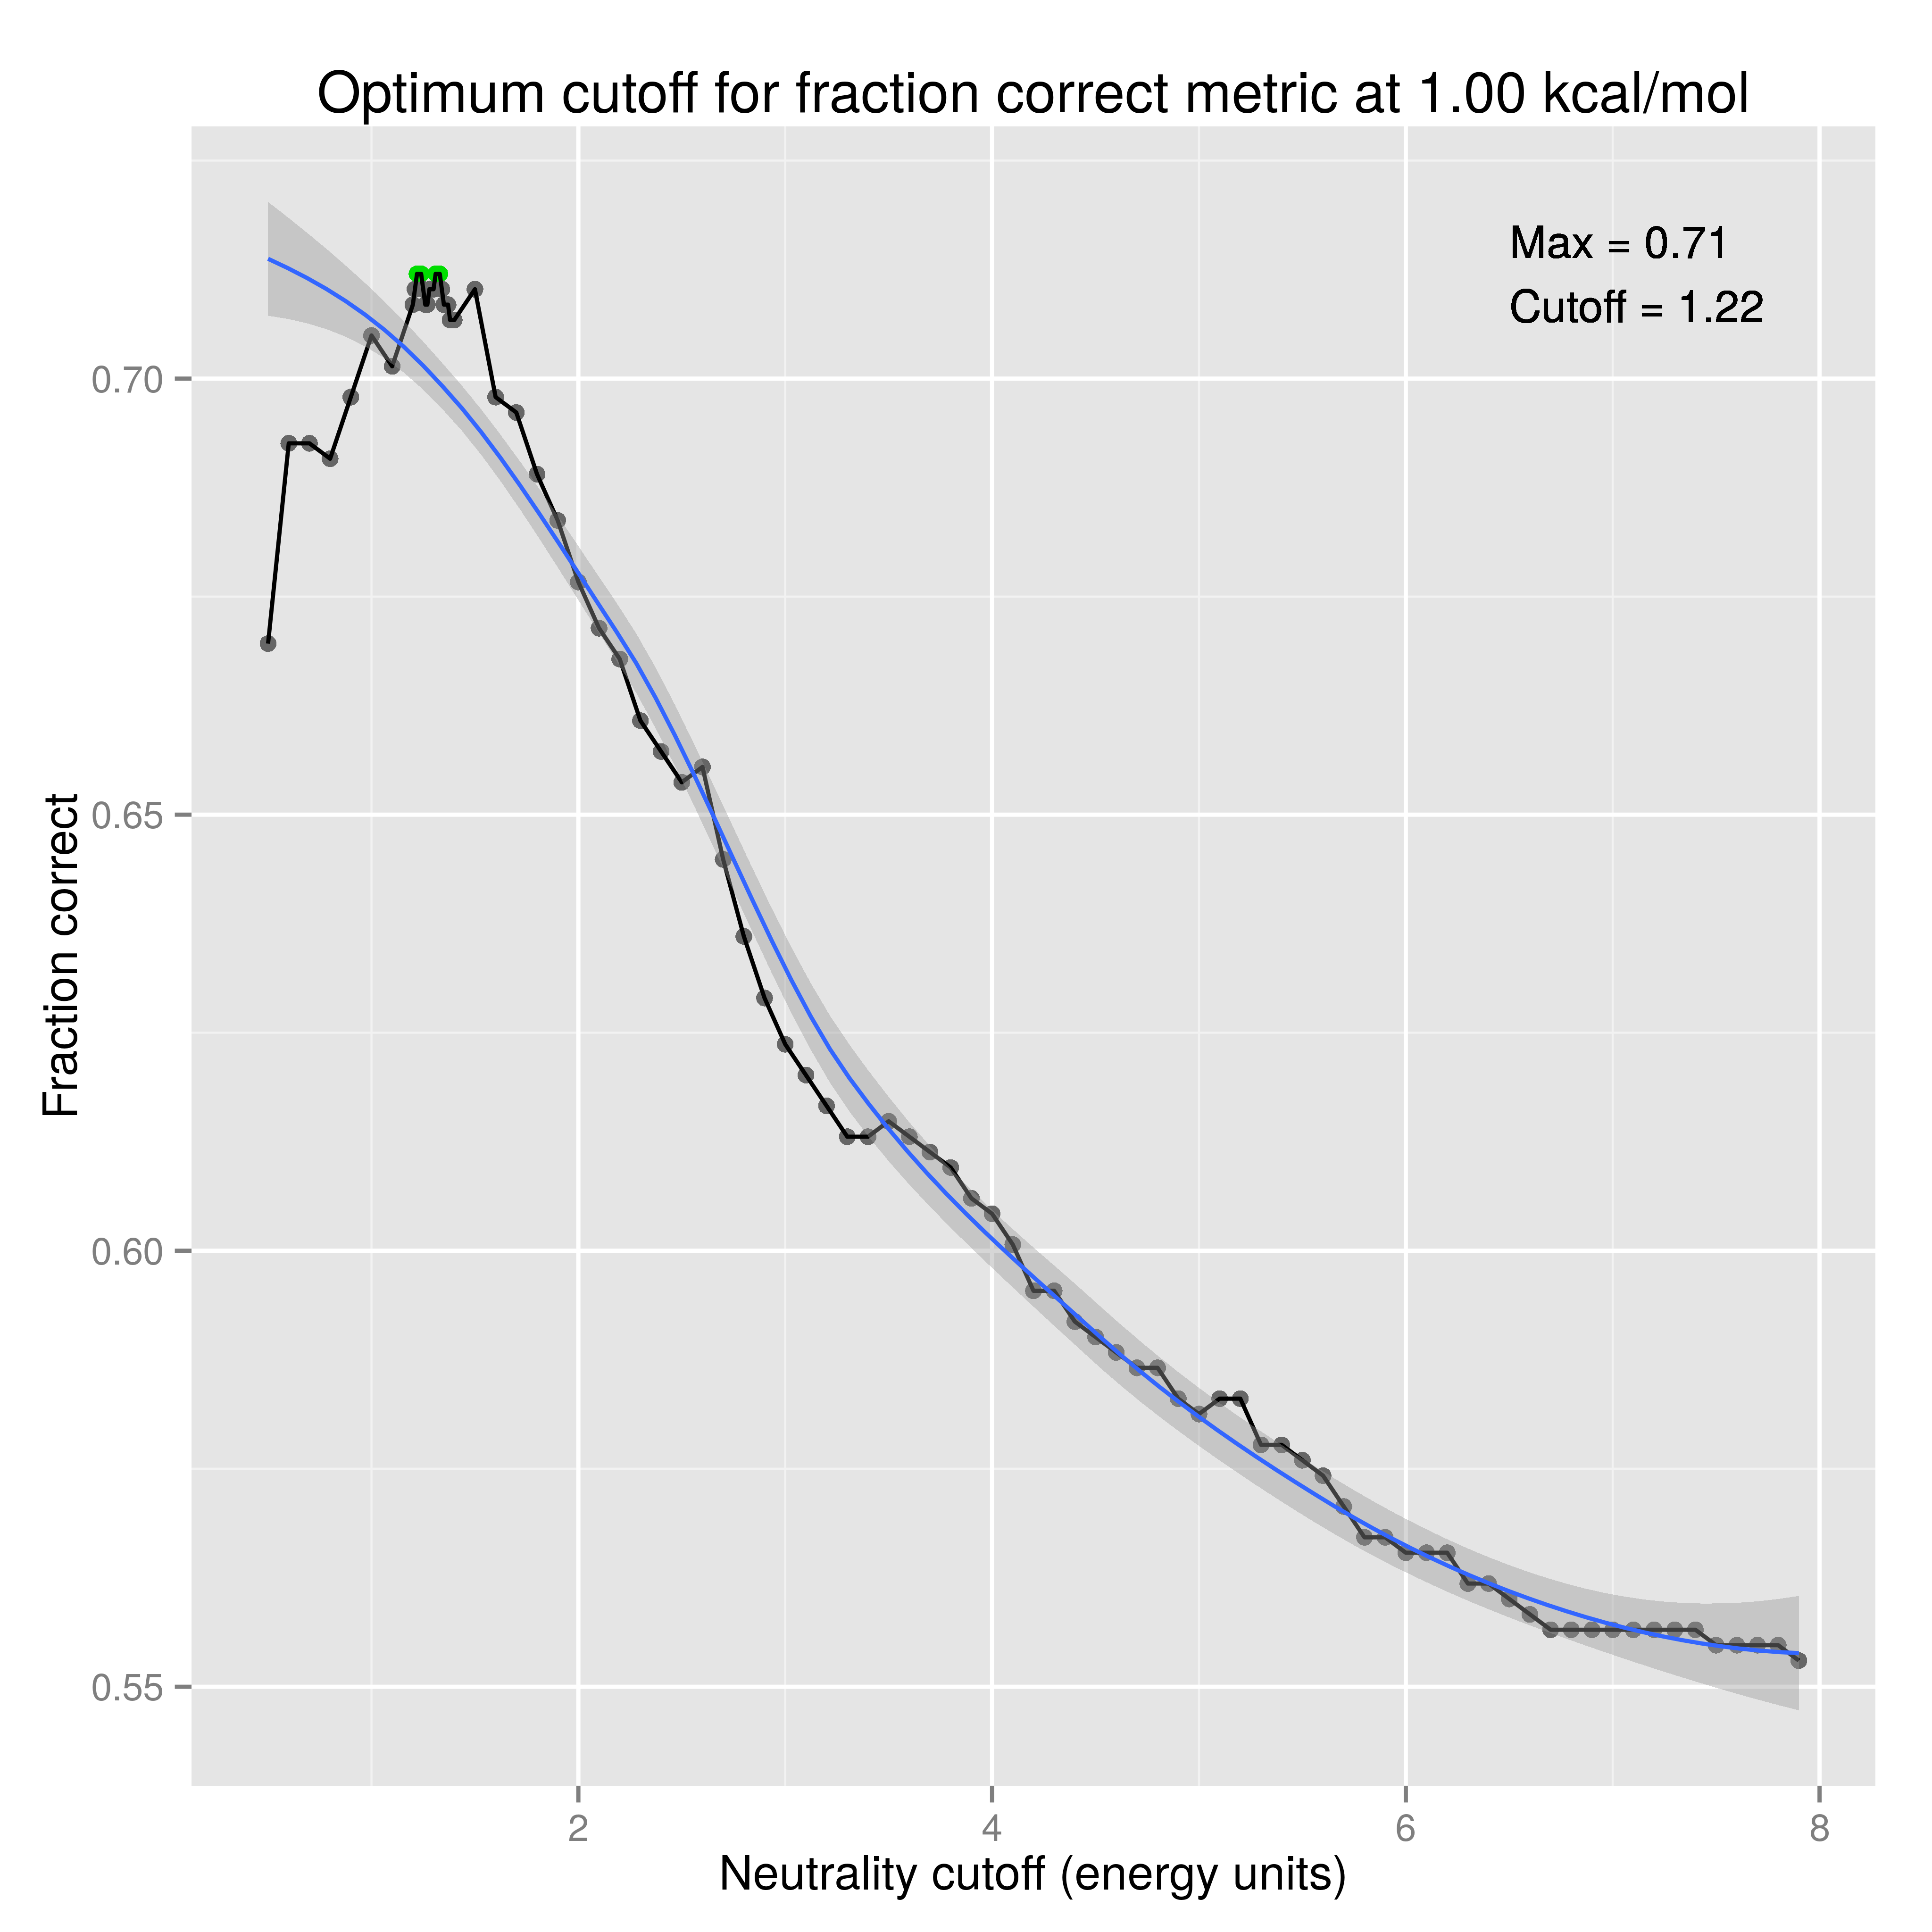
\includegraphics[width=\textwidth]{{/tmp/kyleb/multiple_analysis/analysis_sets/ZEMu/topx_1-prediction_set_id_zemu-values-score_method_zemu-paper/zemu-values_subplots/zemu-values_ZEMu_optimum_fraction_correct_at_1.00_kcal_mol}.png}
  \caption{Optimal predictive cutoff plot}
\end{figure}
\begin{figure}[H]
  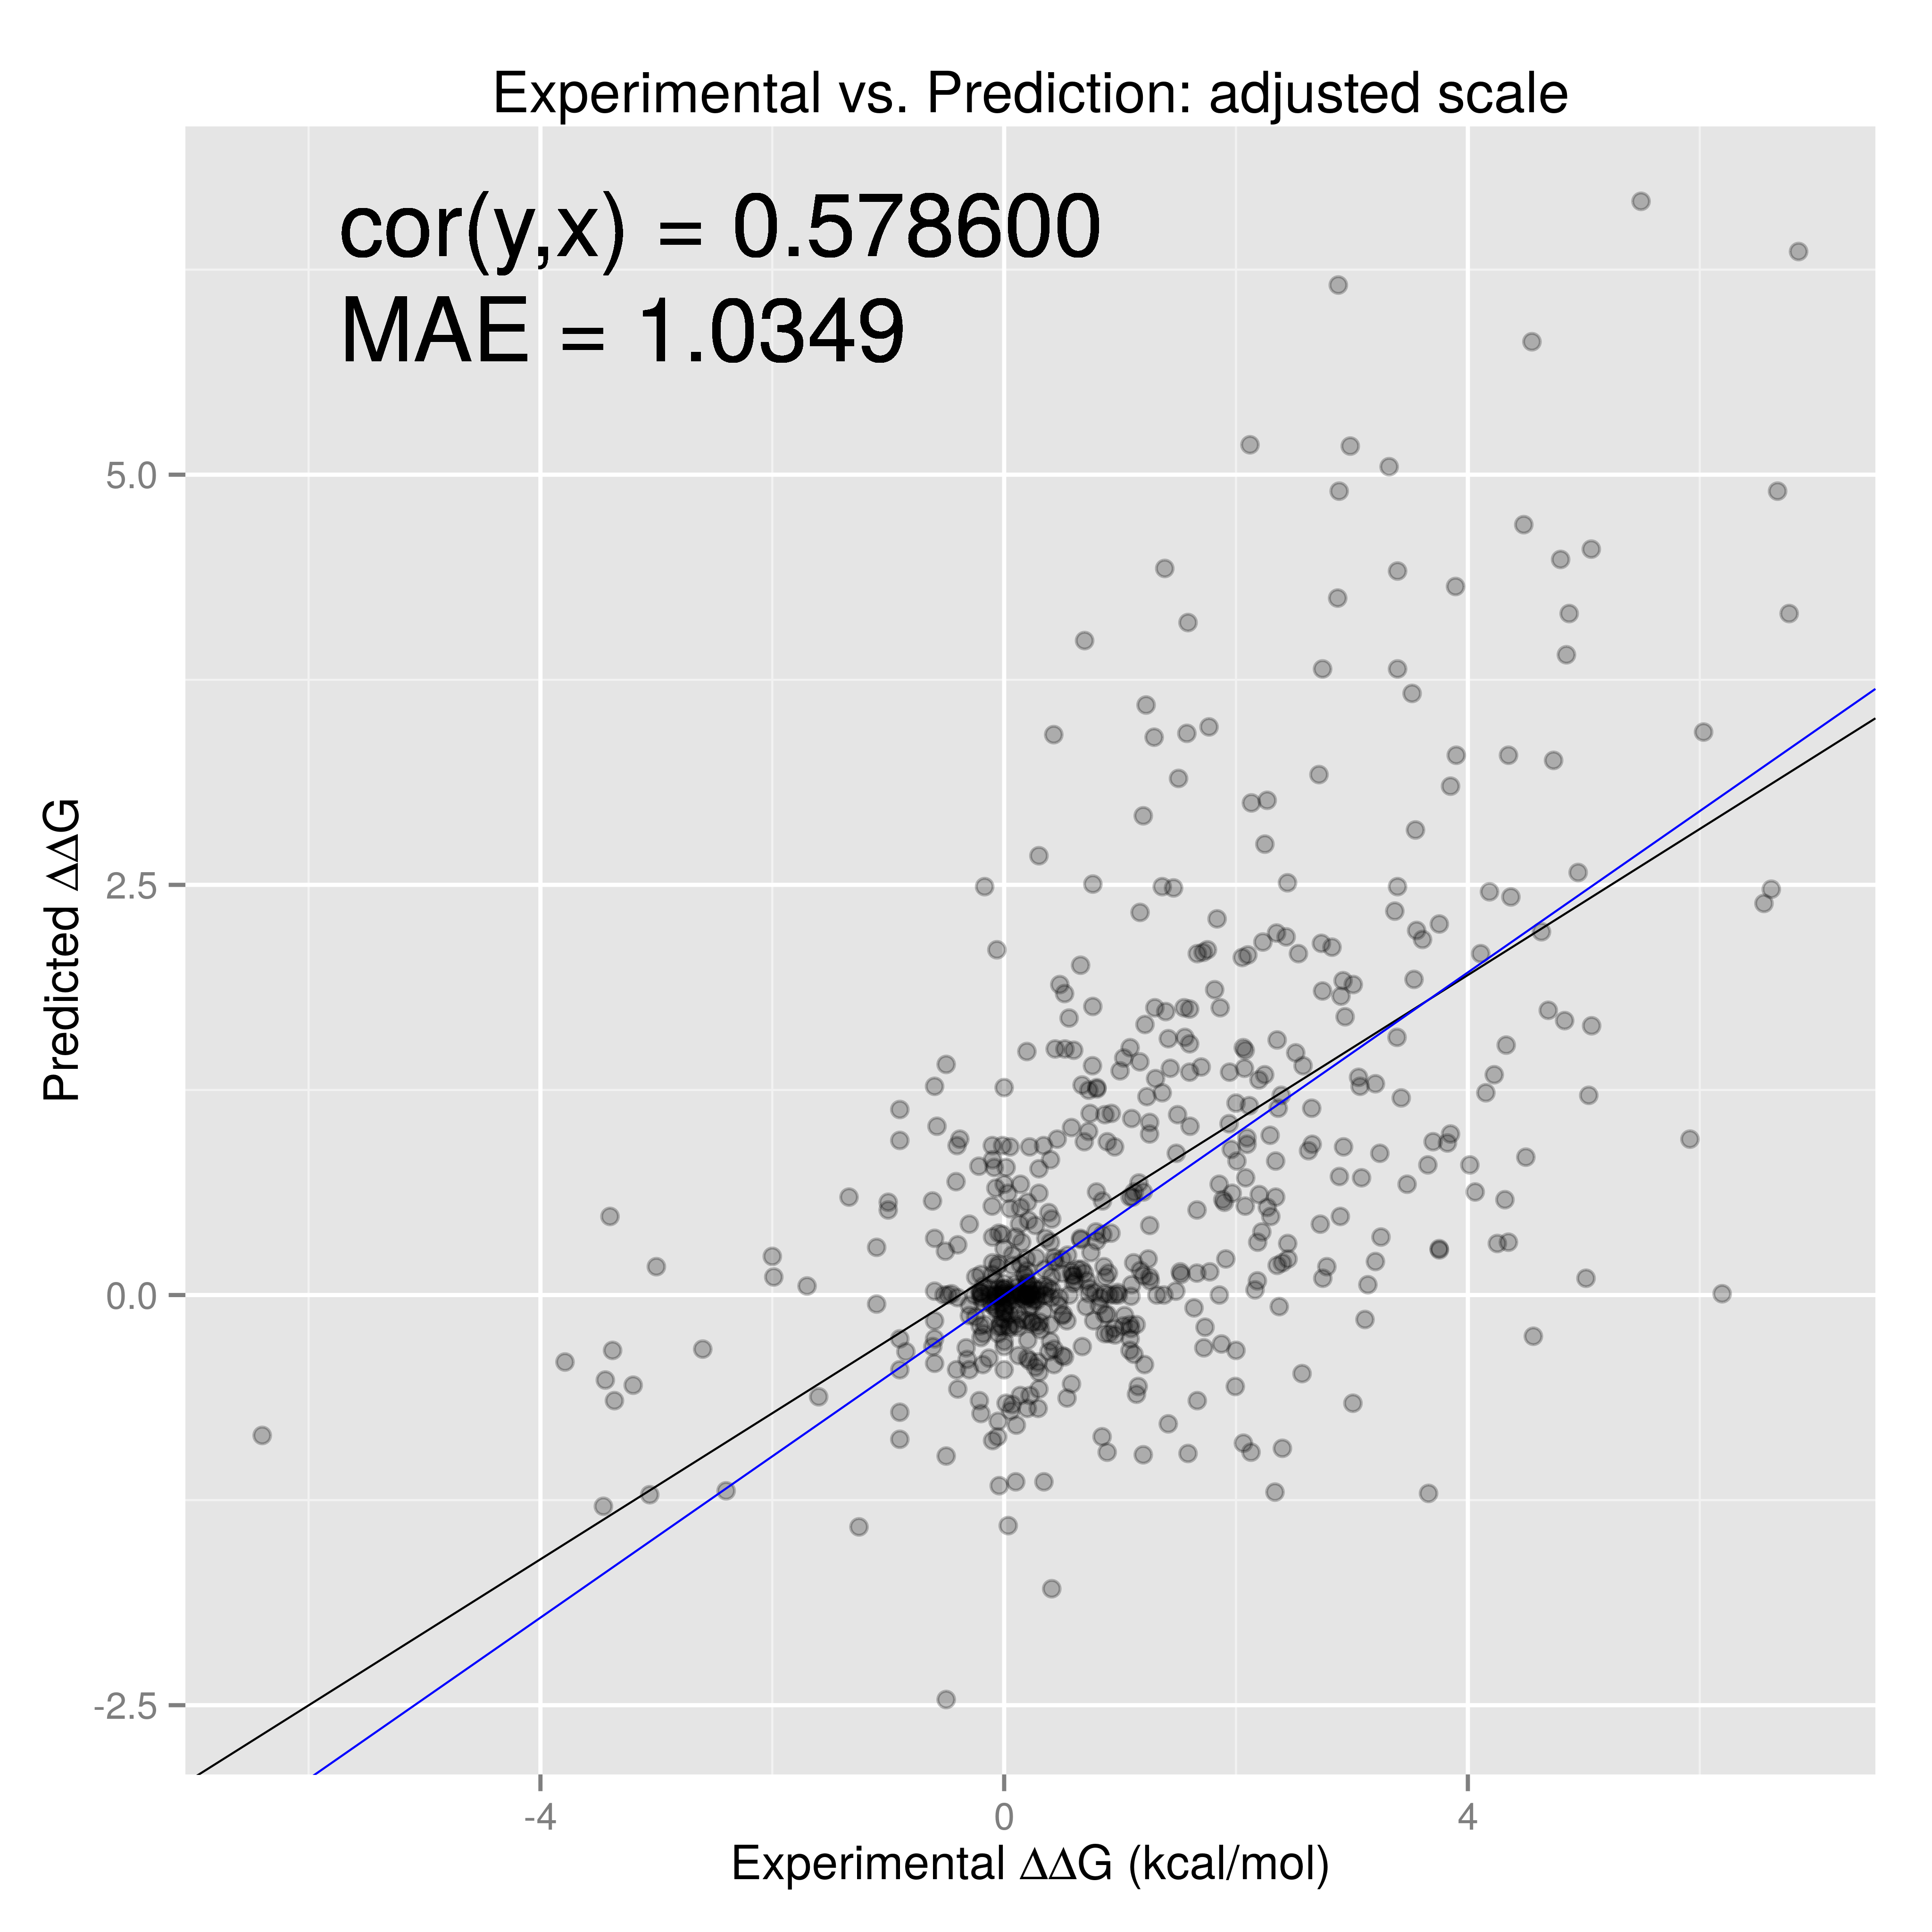
\includegraphics[width=\textwidth]{{/tmp/kyleb/multiple_analysis/analysis_sets/ZEMu/topx_1-prediction_set_id_zemu-values-score_method_zemu-paper/zemu-values_subplots/zemu-values_ZEMu_main_adjusted_with_scalar_scatterplot}.png}
  \caption{Main adj. scatterplot}
\end{figure}
\begin{figure}[H]
  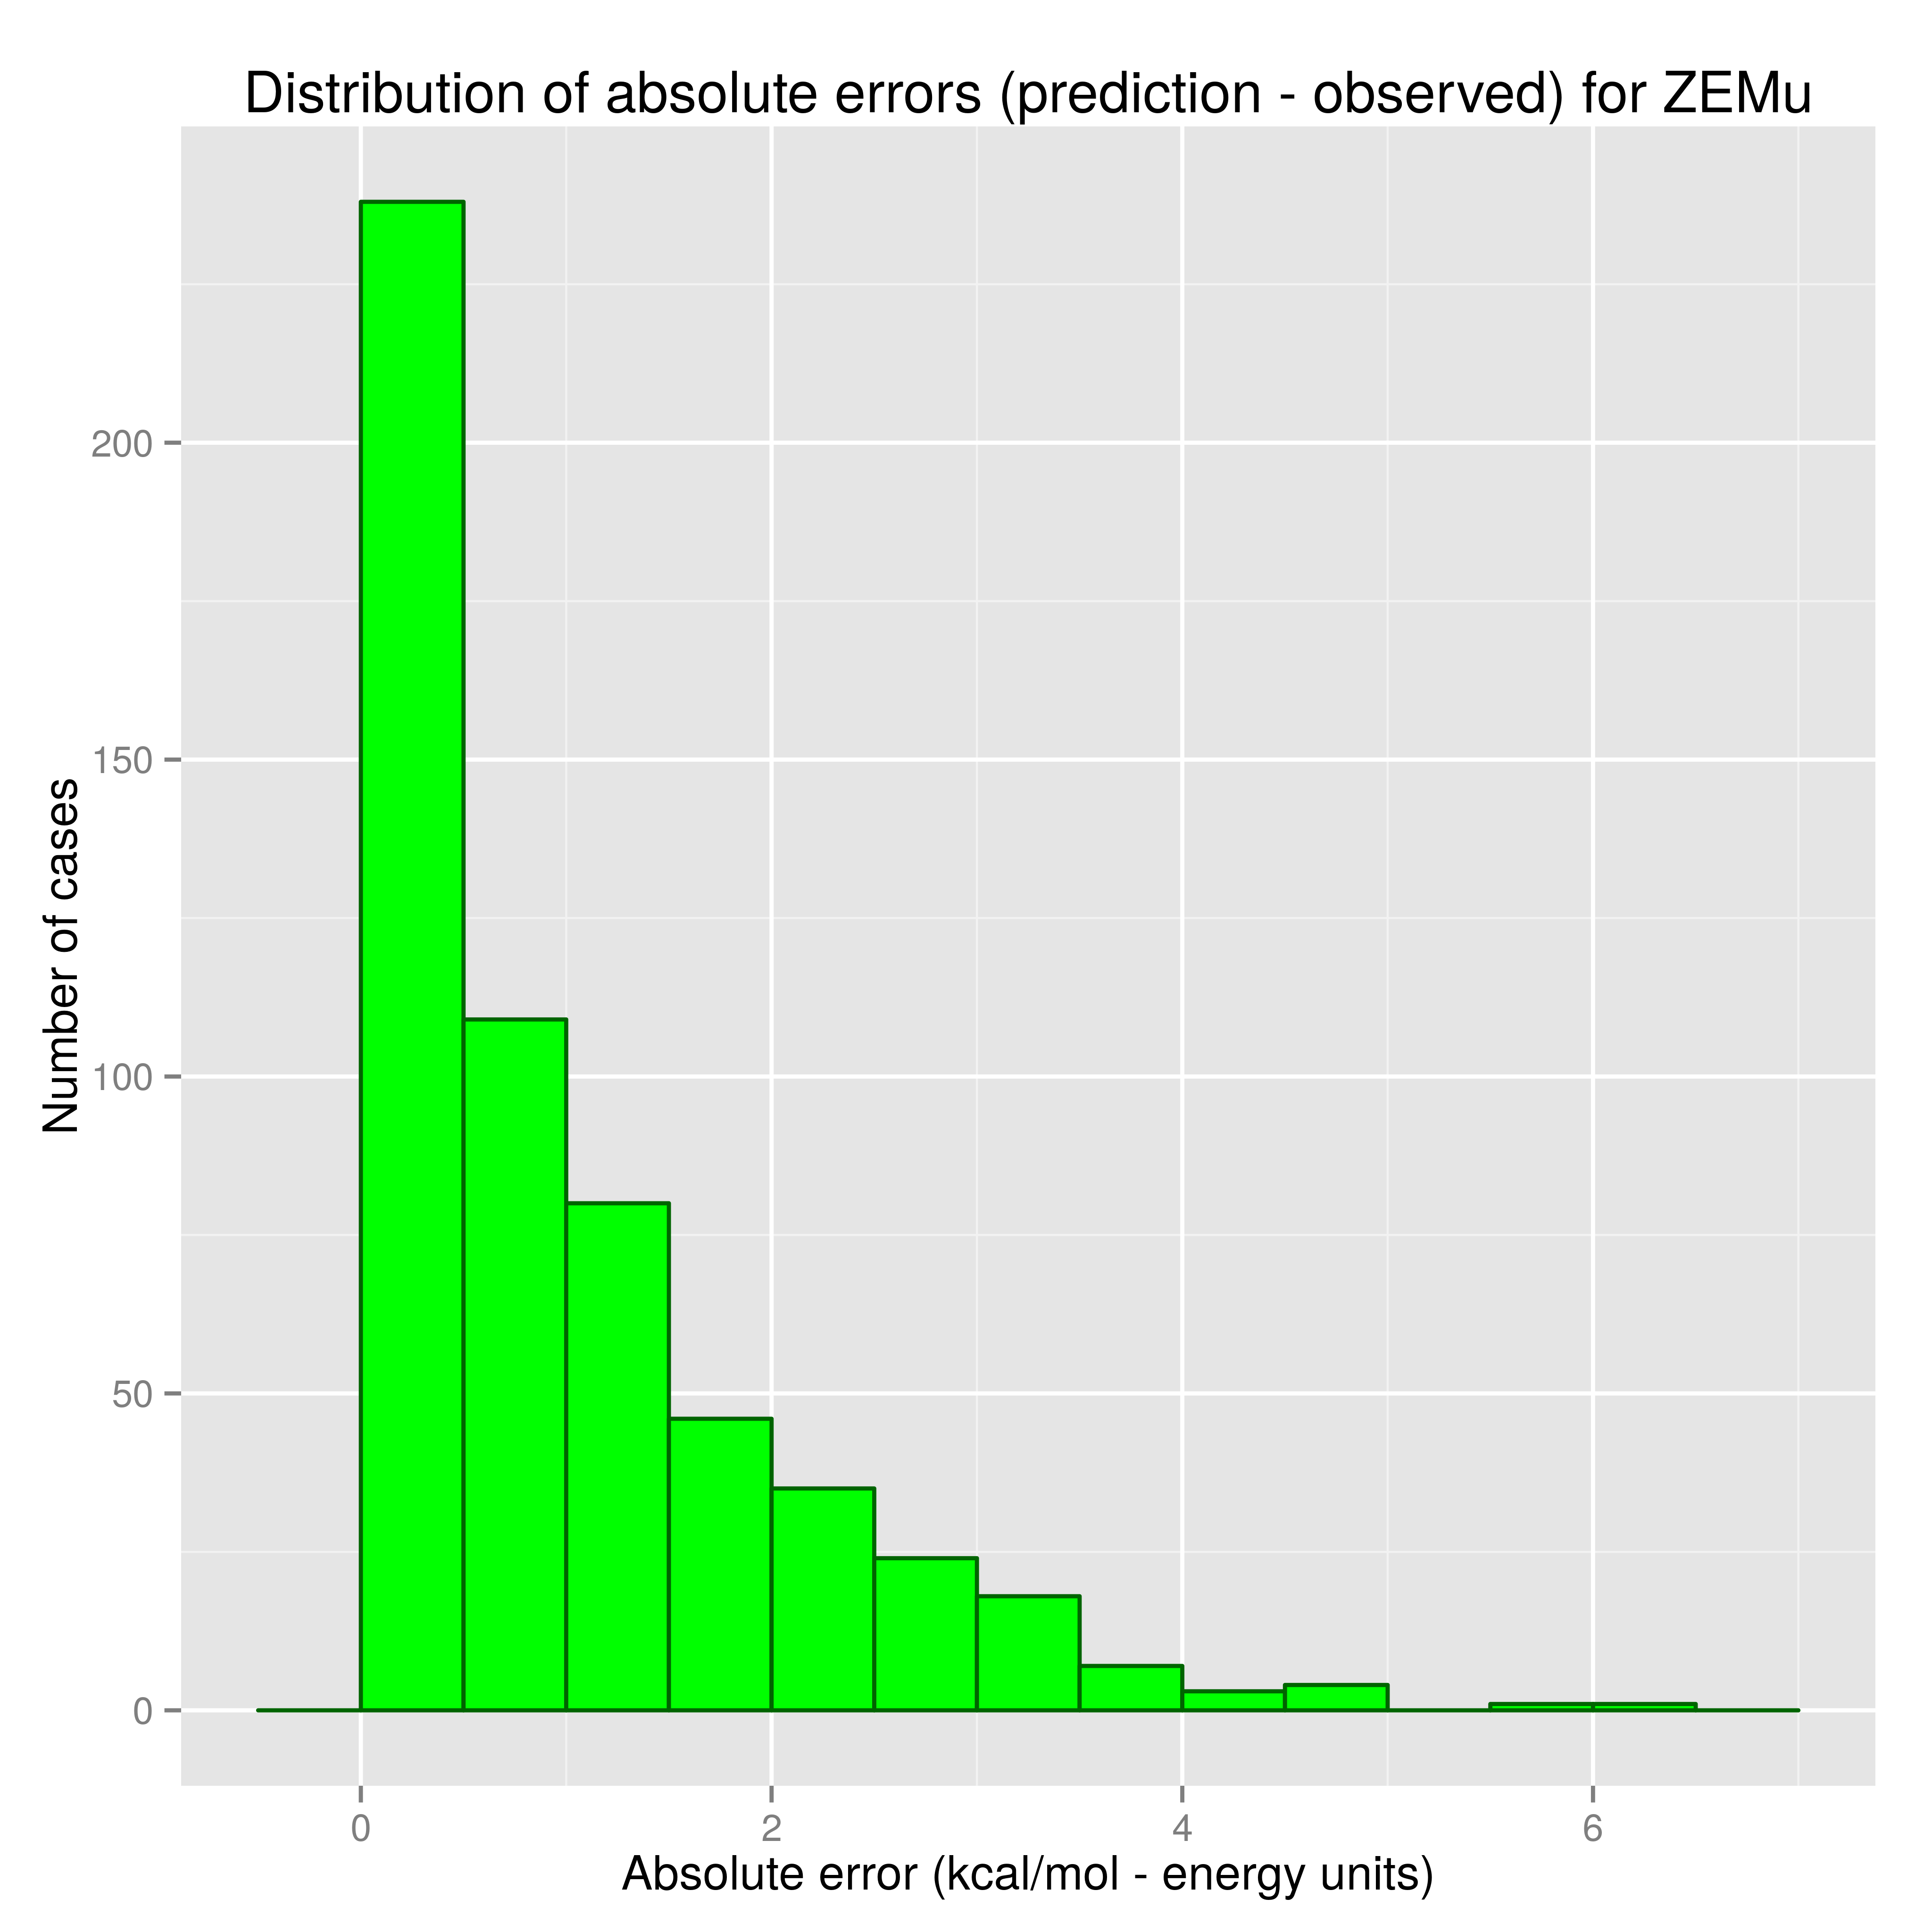
\includegraphics[width=\textwidth]{{/tmp/kyleb/multiple_analysis/analysis_sets/ZEMu/topx_1-prediction_set_id_zemu-values-score_method_zemu-paper/zemu-values_subplots/zemu-values_ZEMu_absolute_errors_adjusted_with_scalar}.png}
  \caption{Absolute errors adjusted with scalar}
\end{figure}

\clearpage

\section{Residue context}

\begin{figure}[H]
  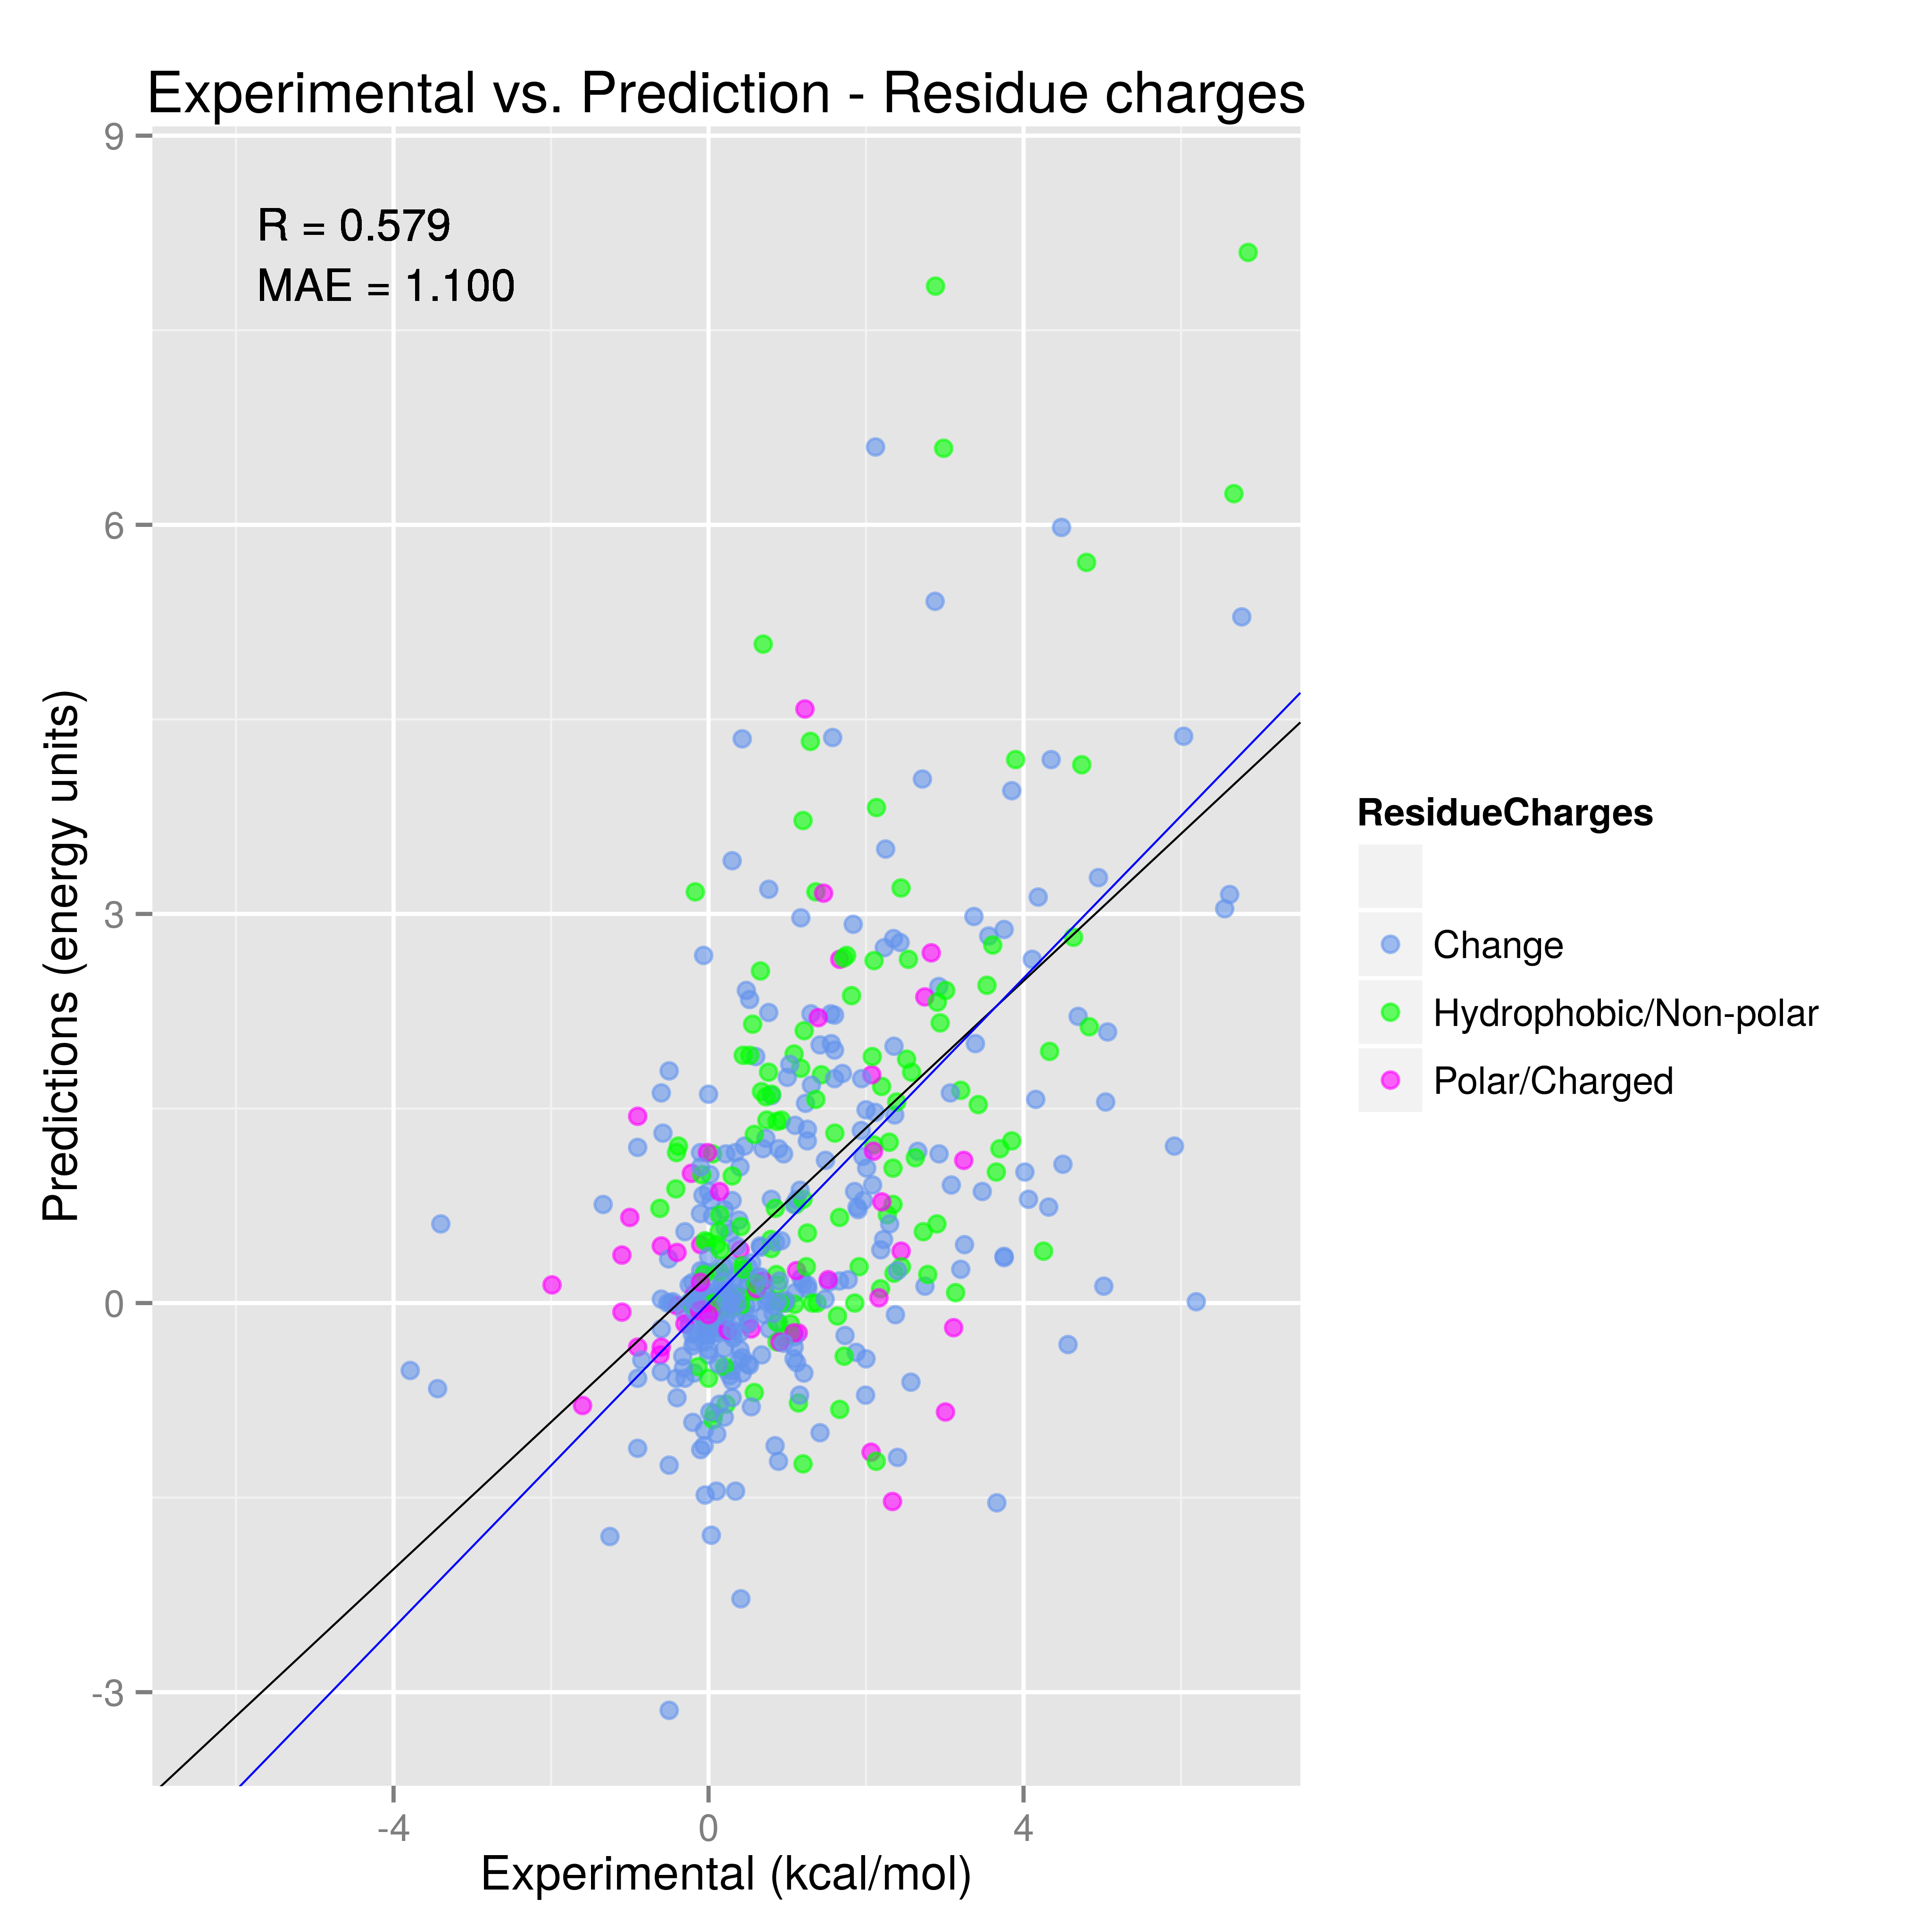
\includegraphics[width=\textwidth]{{/tmp/kyleb/multiple_analysis/analysis_sets/ZEMu/topx_1-prediction_set_id_zemu-values-score_method_zemu-paper/zemu-values_subplots/zemu-values_ZEMu_scatterplot_charges}.png}
  \caption{Experimental vs. Prediction - Residue charges}
\end{figure}
\begin{figure}[H]
  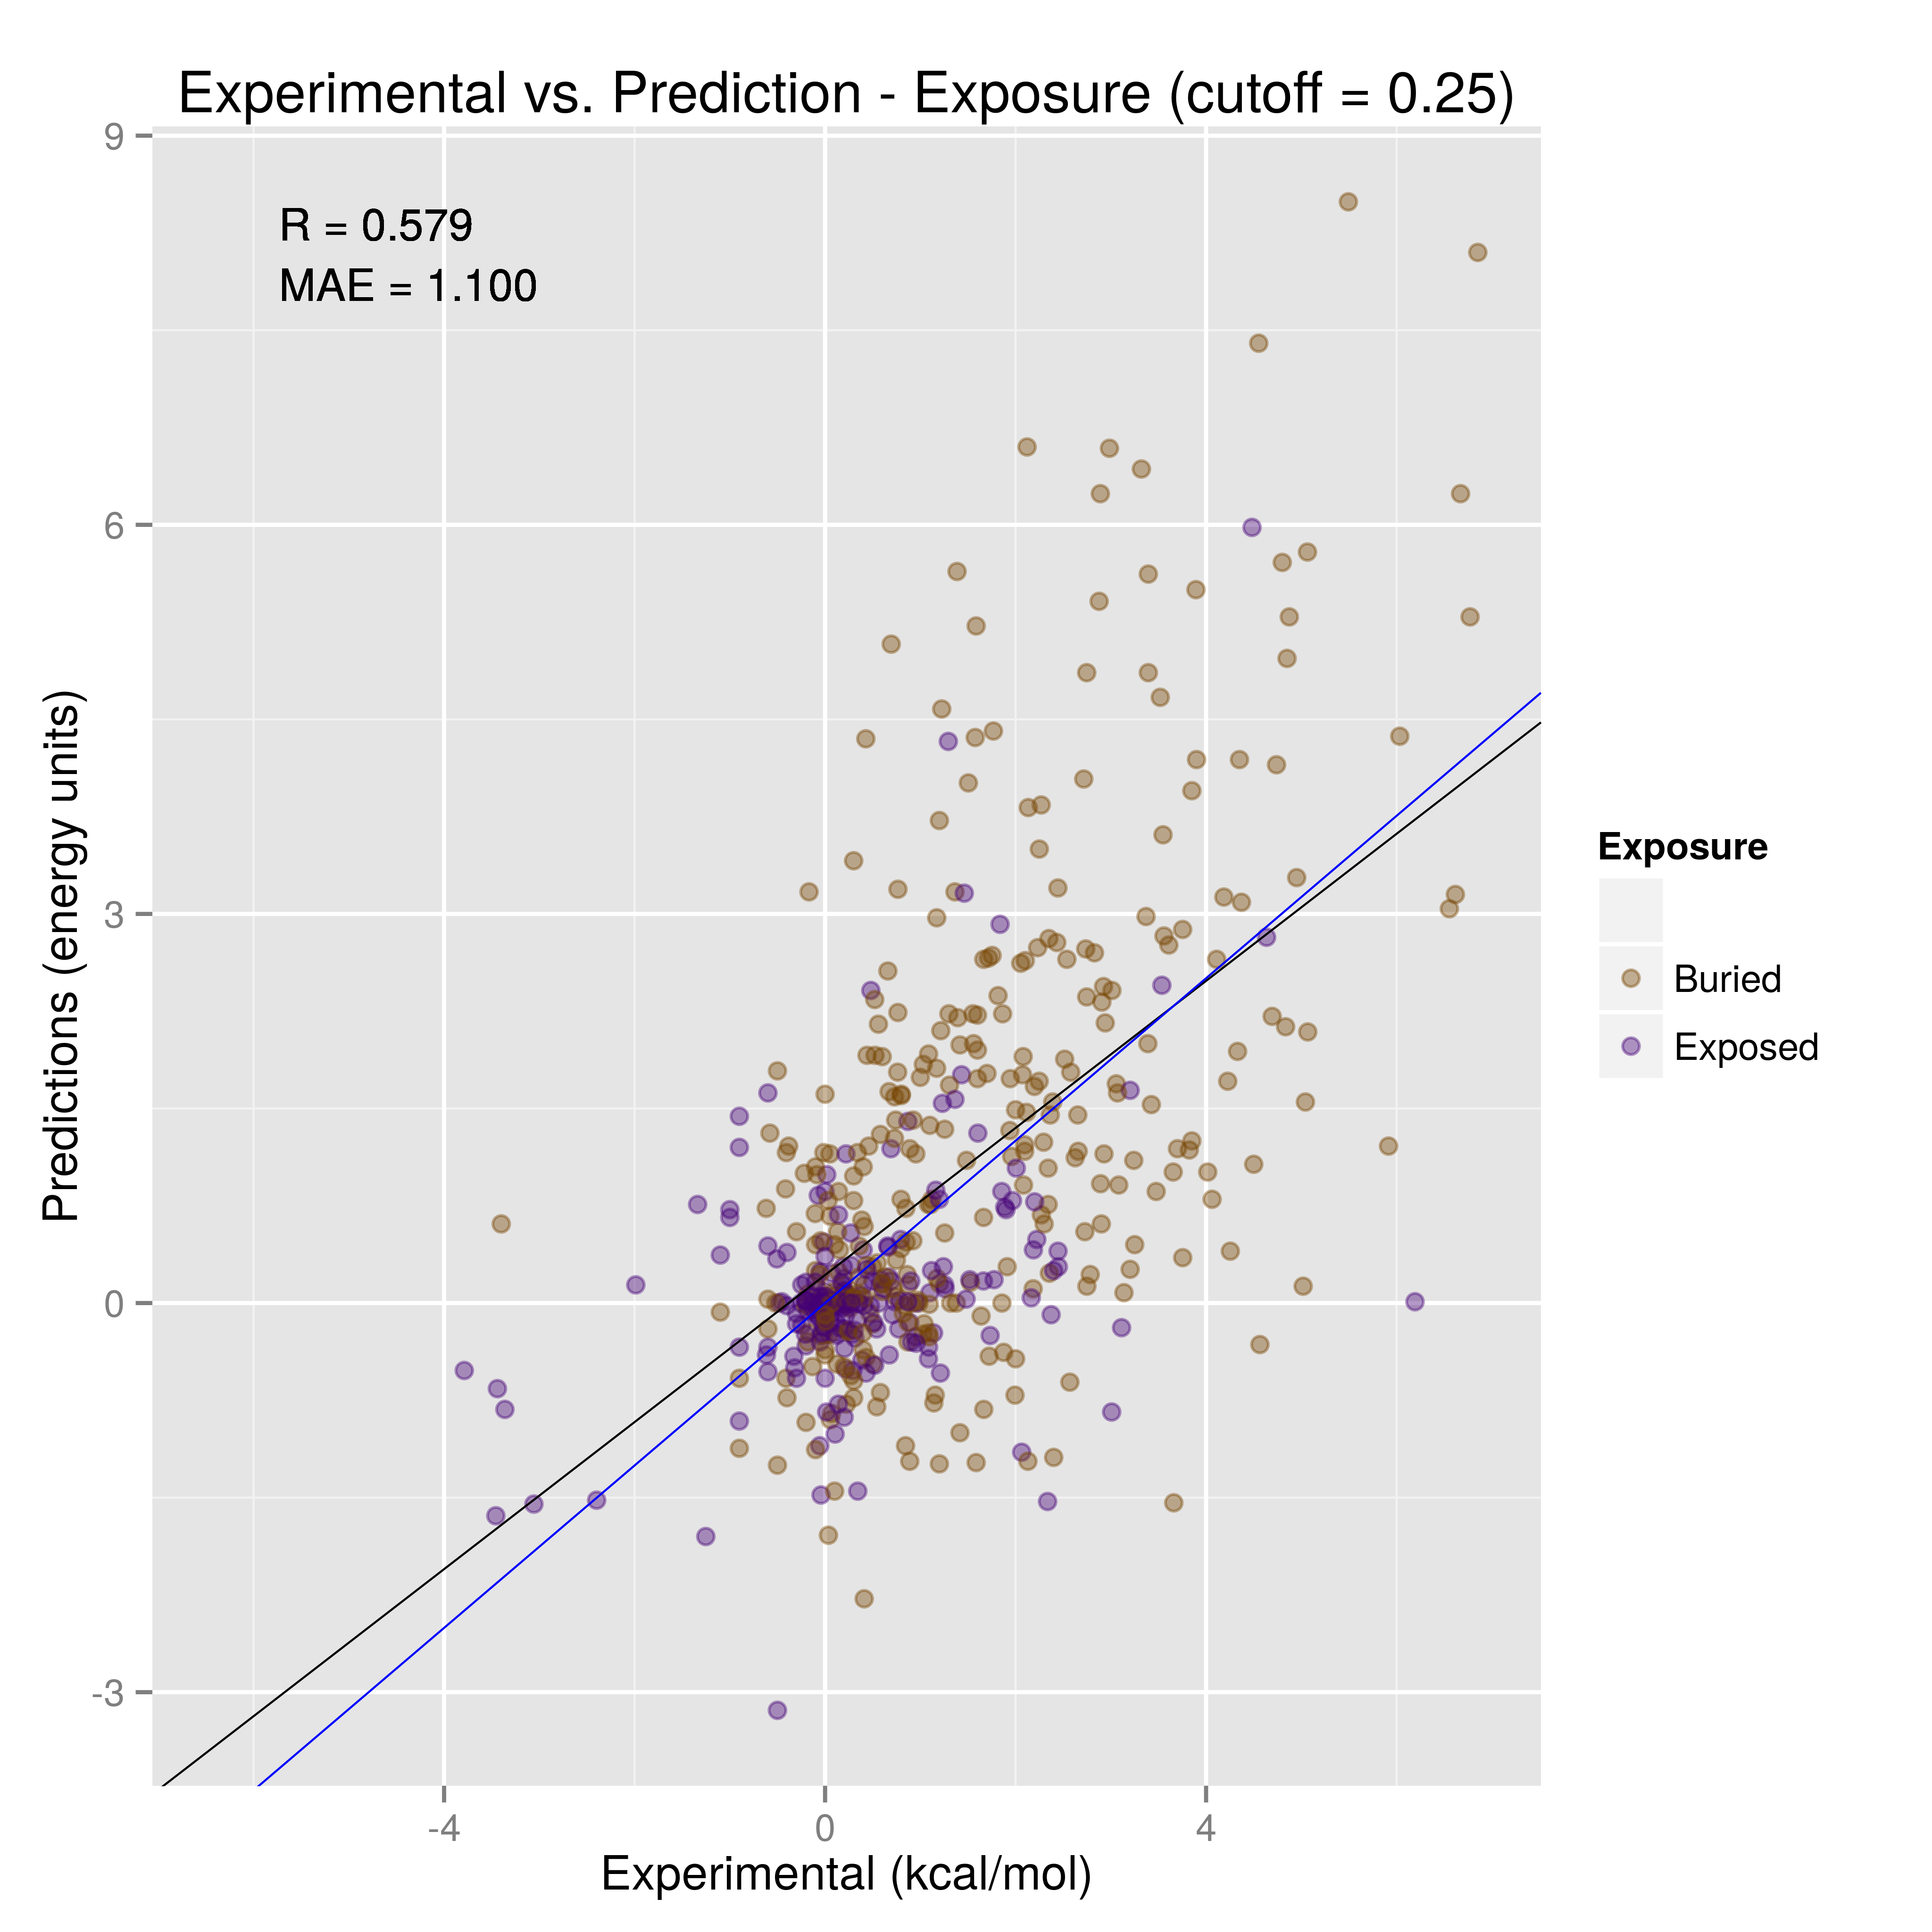
\includegraphics[width=\textwidth]{{/tmp/kyleb/multiple_analysis/analysis_sets/ZEMu/topx_1-prediction_set_id_zemu-values-score_method_zemu-paper/zemu-values_subplots/zemu-values_ZEMu_scatterplot_exposure}.png}
  \caption{Experimental vs. Prediction - Exposure (cutoff = 0.25)}
\end{figure}
\begin{figure}[H]
  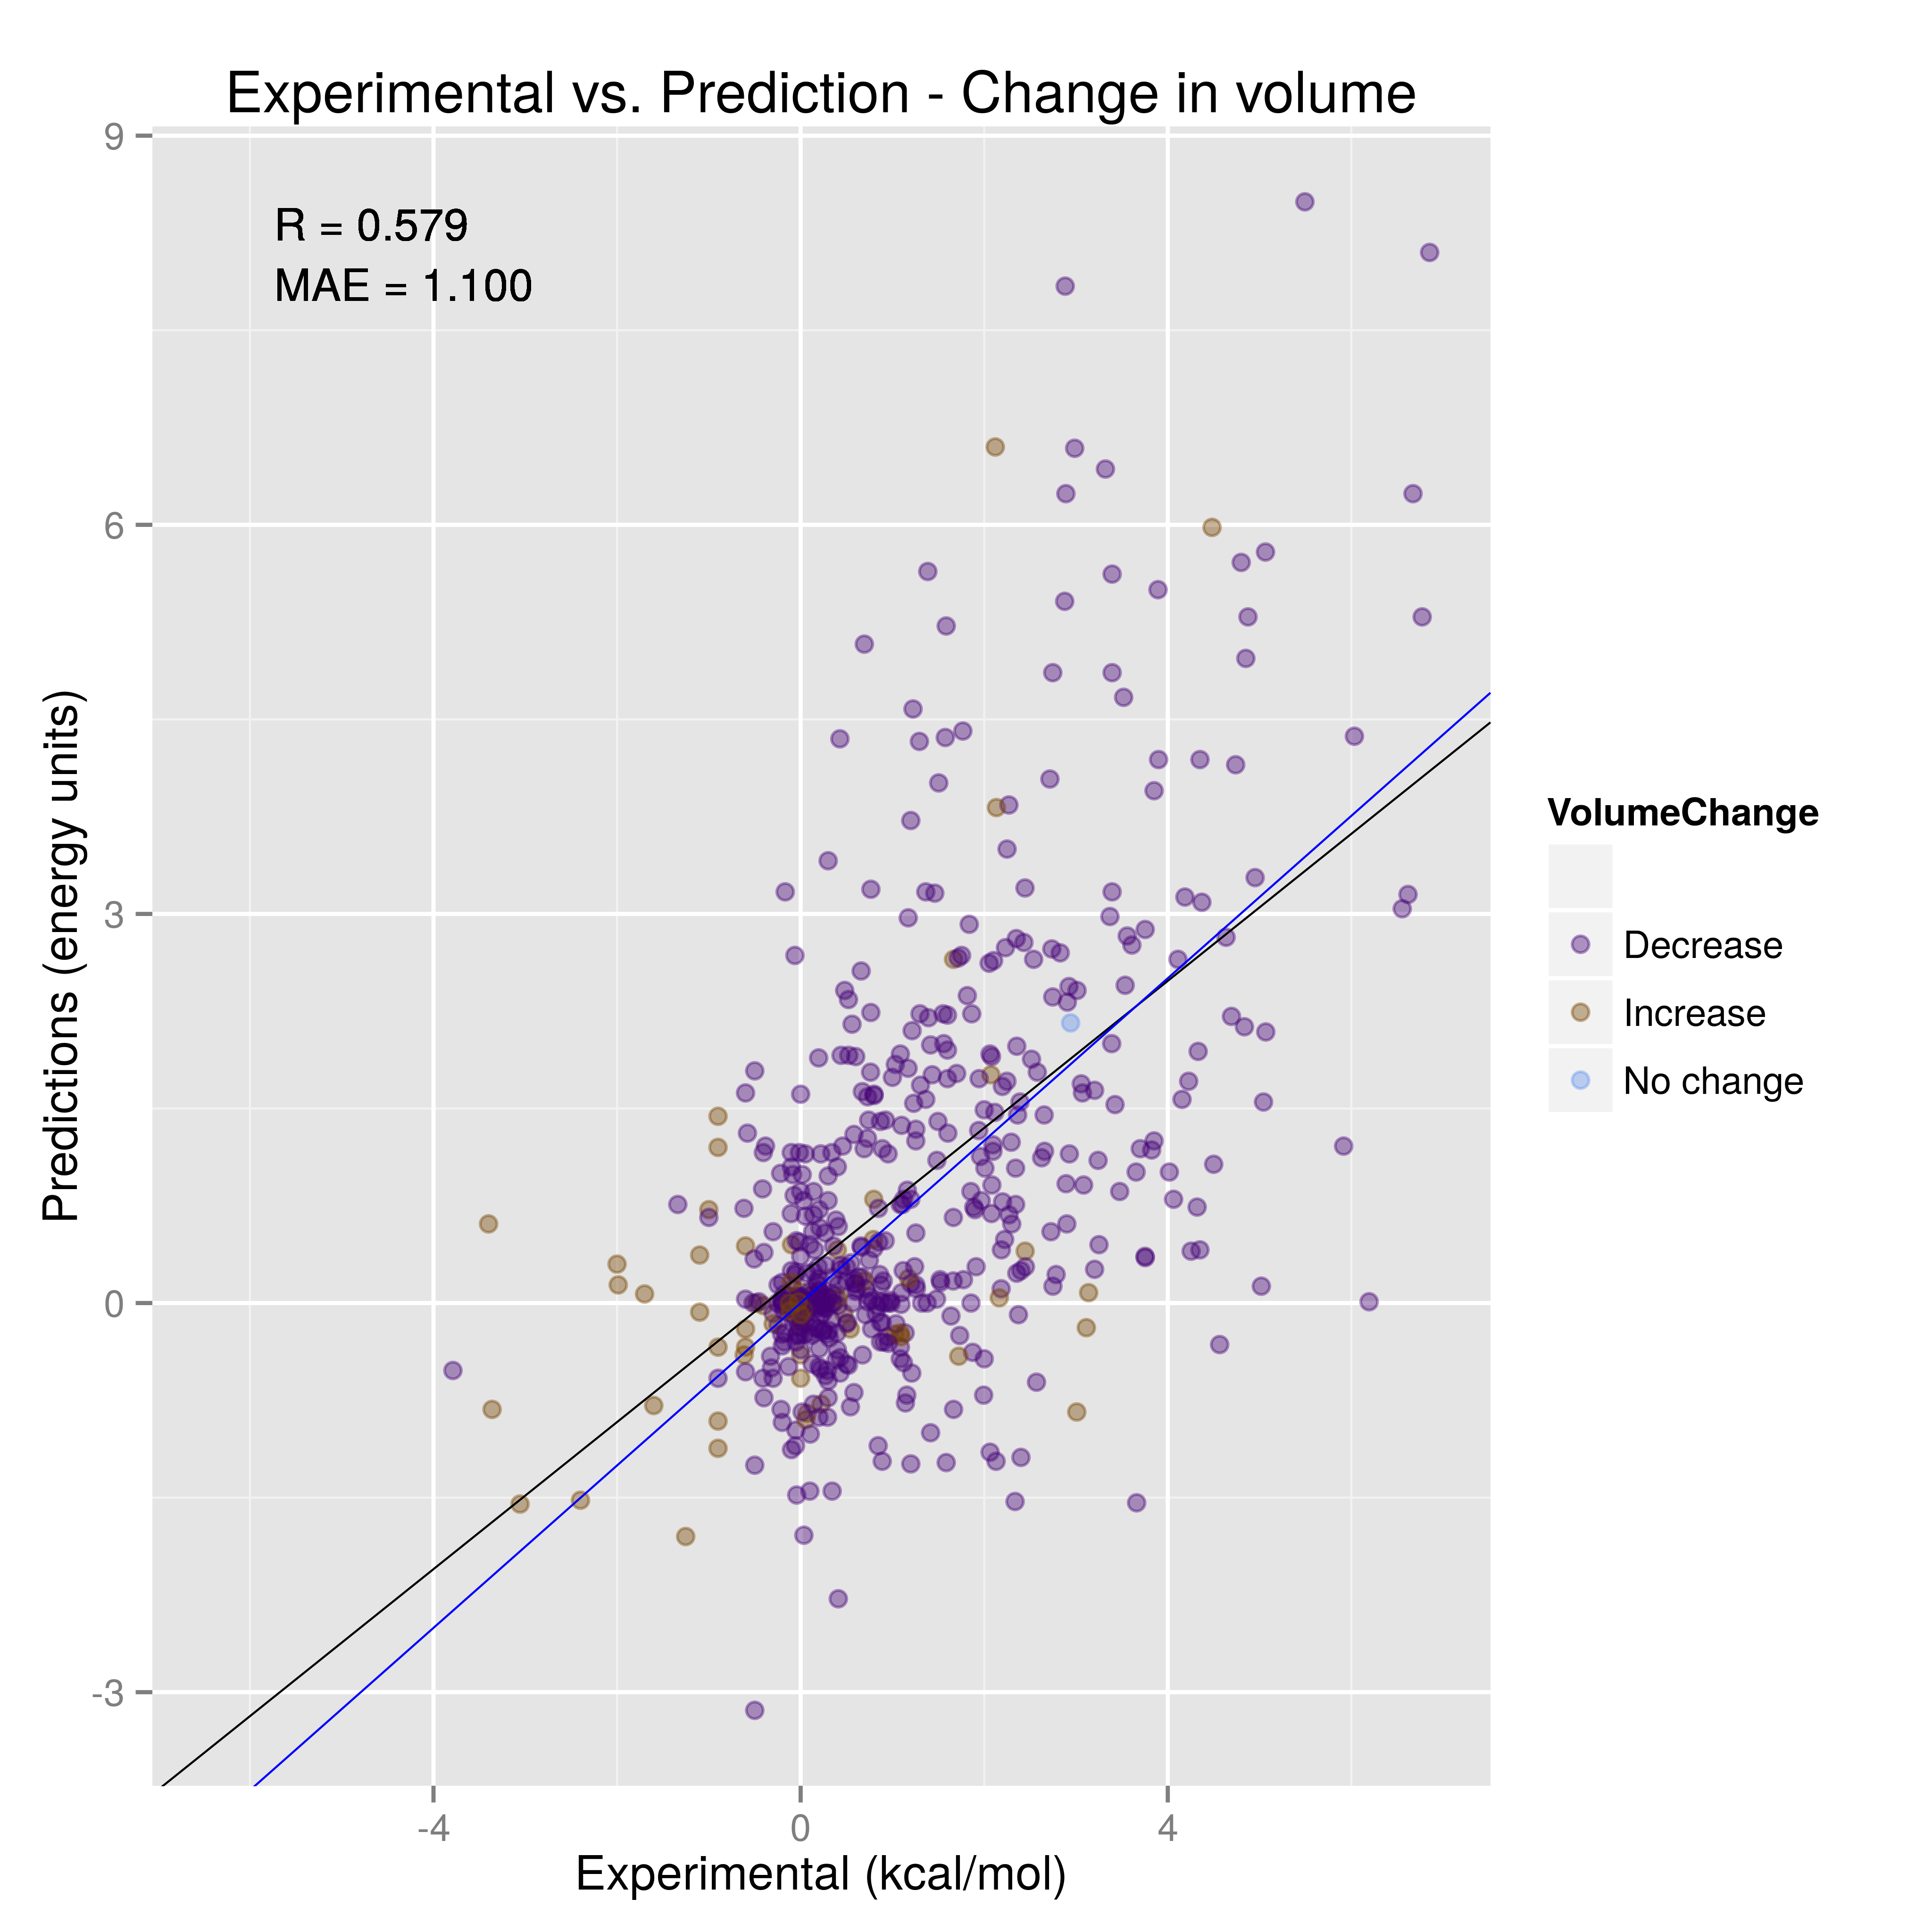
\includegraphics[width=\textwidth]{{/tmp/kyleb/multiple_analysis/analysis_sets/ZEMu/topx_1-prediction_set_id_zemu-values-score_method_zemu-paper/zemu-values_subplots/zemu-values_ZEMu_scatterplot_volume}.png}
  \caption{Experimental vs. Prediction - Change in volume}
\end{figure}
\begin{figure}[H]
  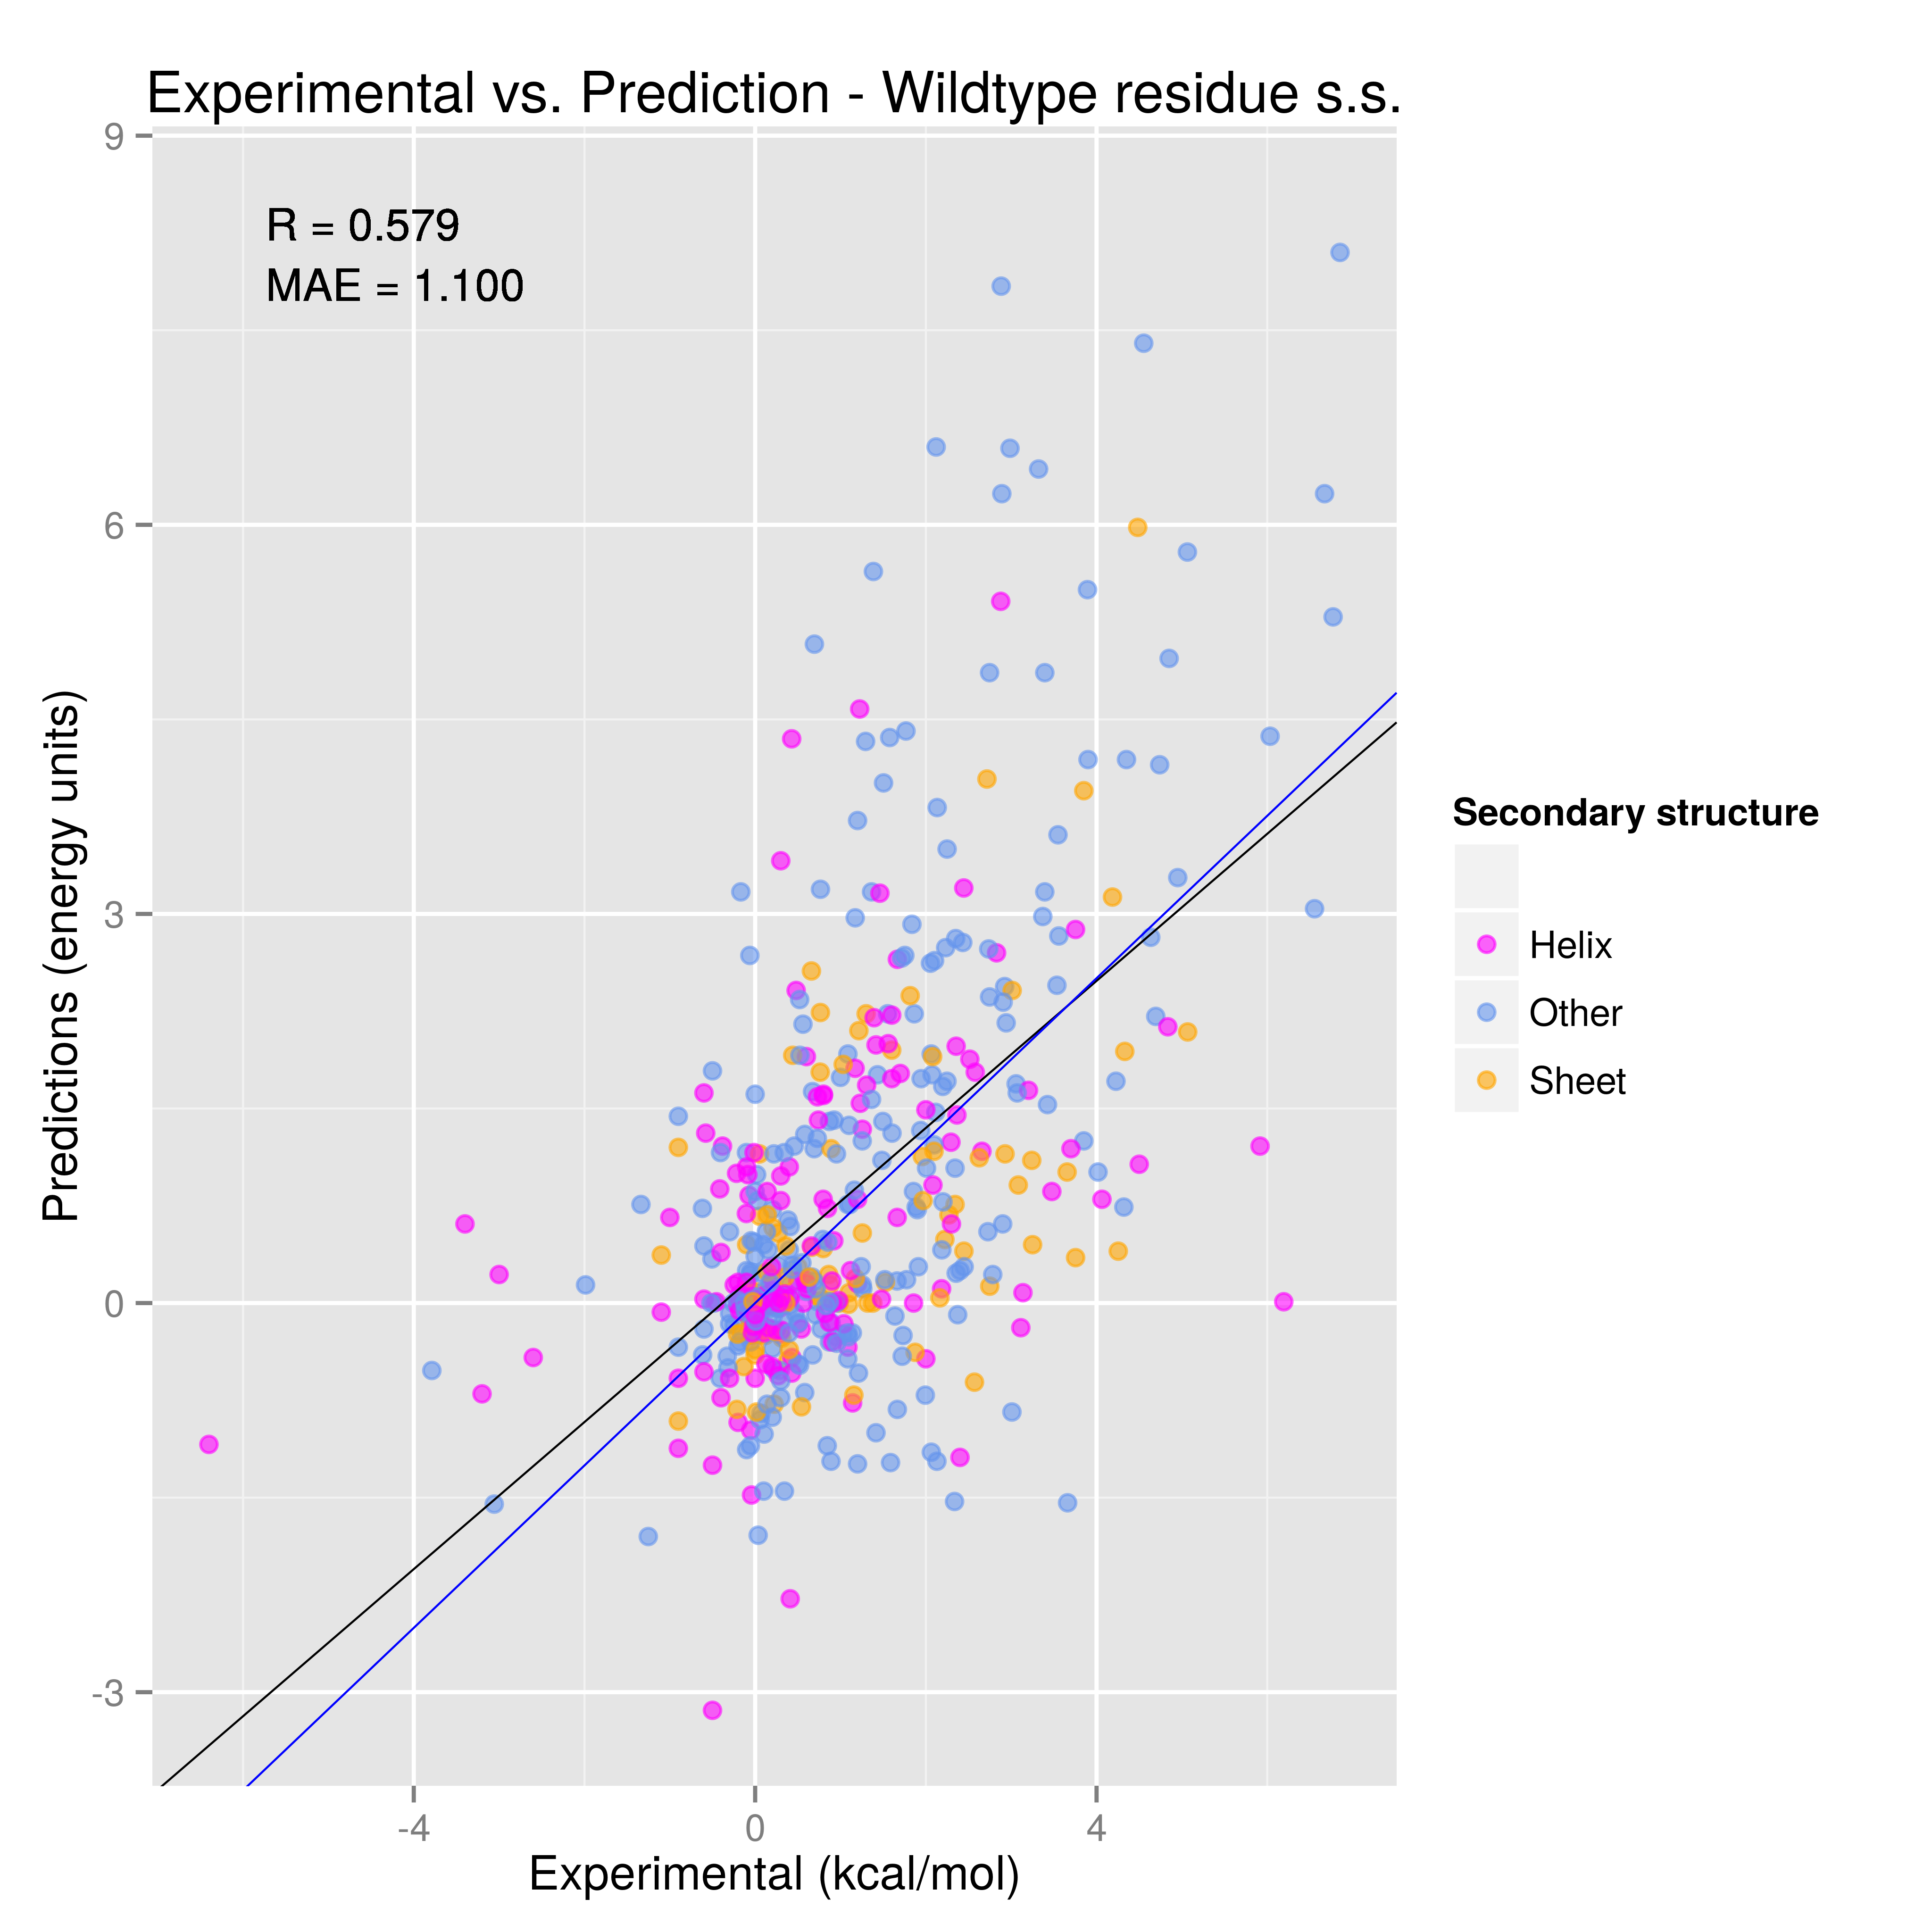
\includegraphics[width=\textwidth]{{/tmp/kyleb/multiple_analysis/analysis_sets/ZEMu/topx_1-prediction_set_id_zemu-values-score_method_zemu-paper/zemu-values_subplots/zemu-values_ZEMu_scatterplot_ss}.png}
  \caption{Experimental vs. Prediction - Wildtype residue s.s.}
\end{figure}

\clearpage

\section{Residue types}

\begin{figure}[H]
  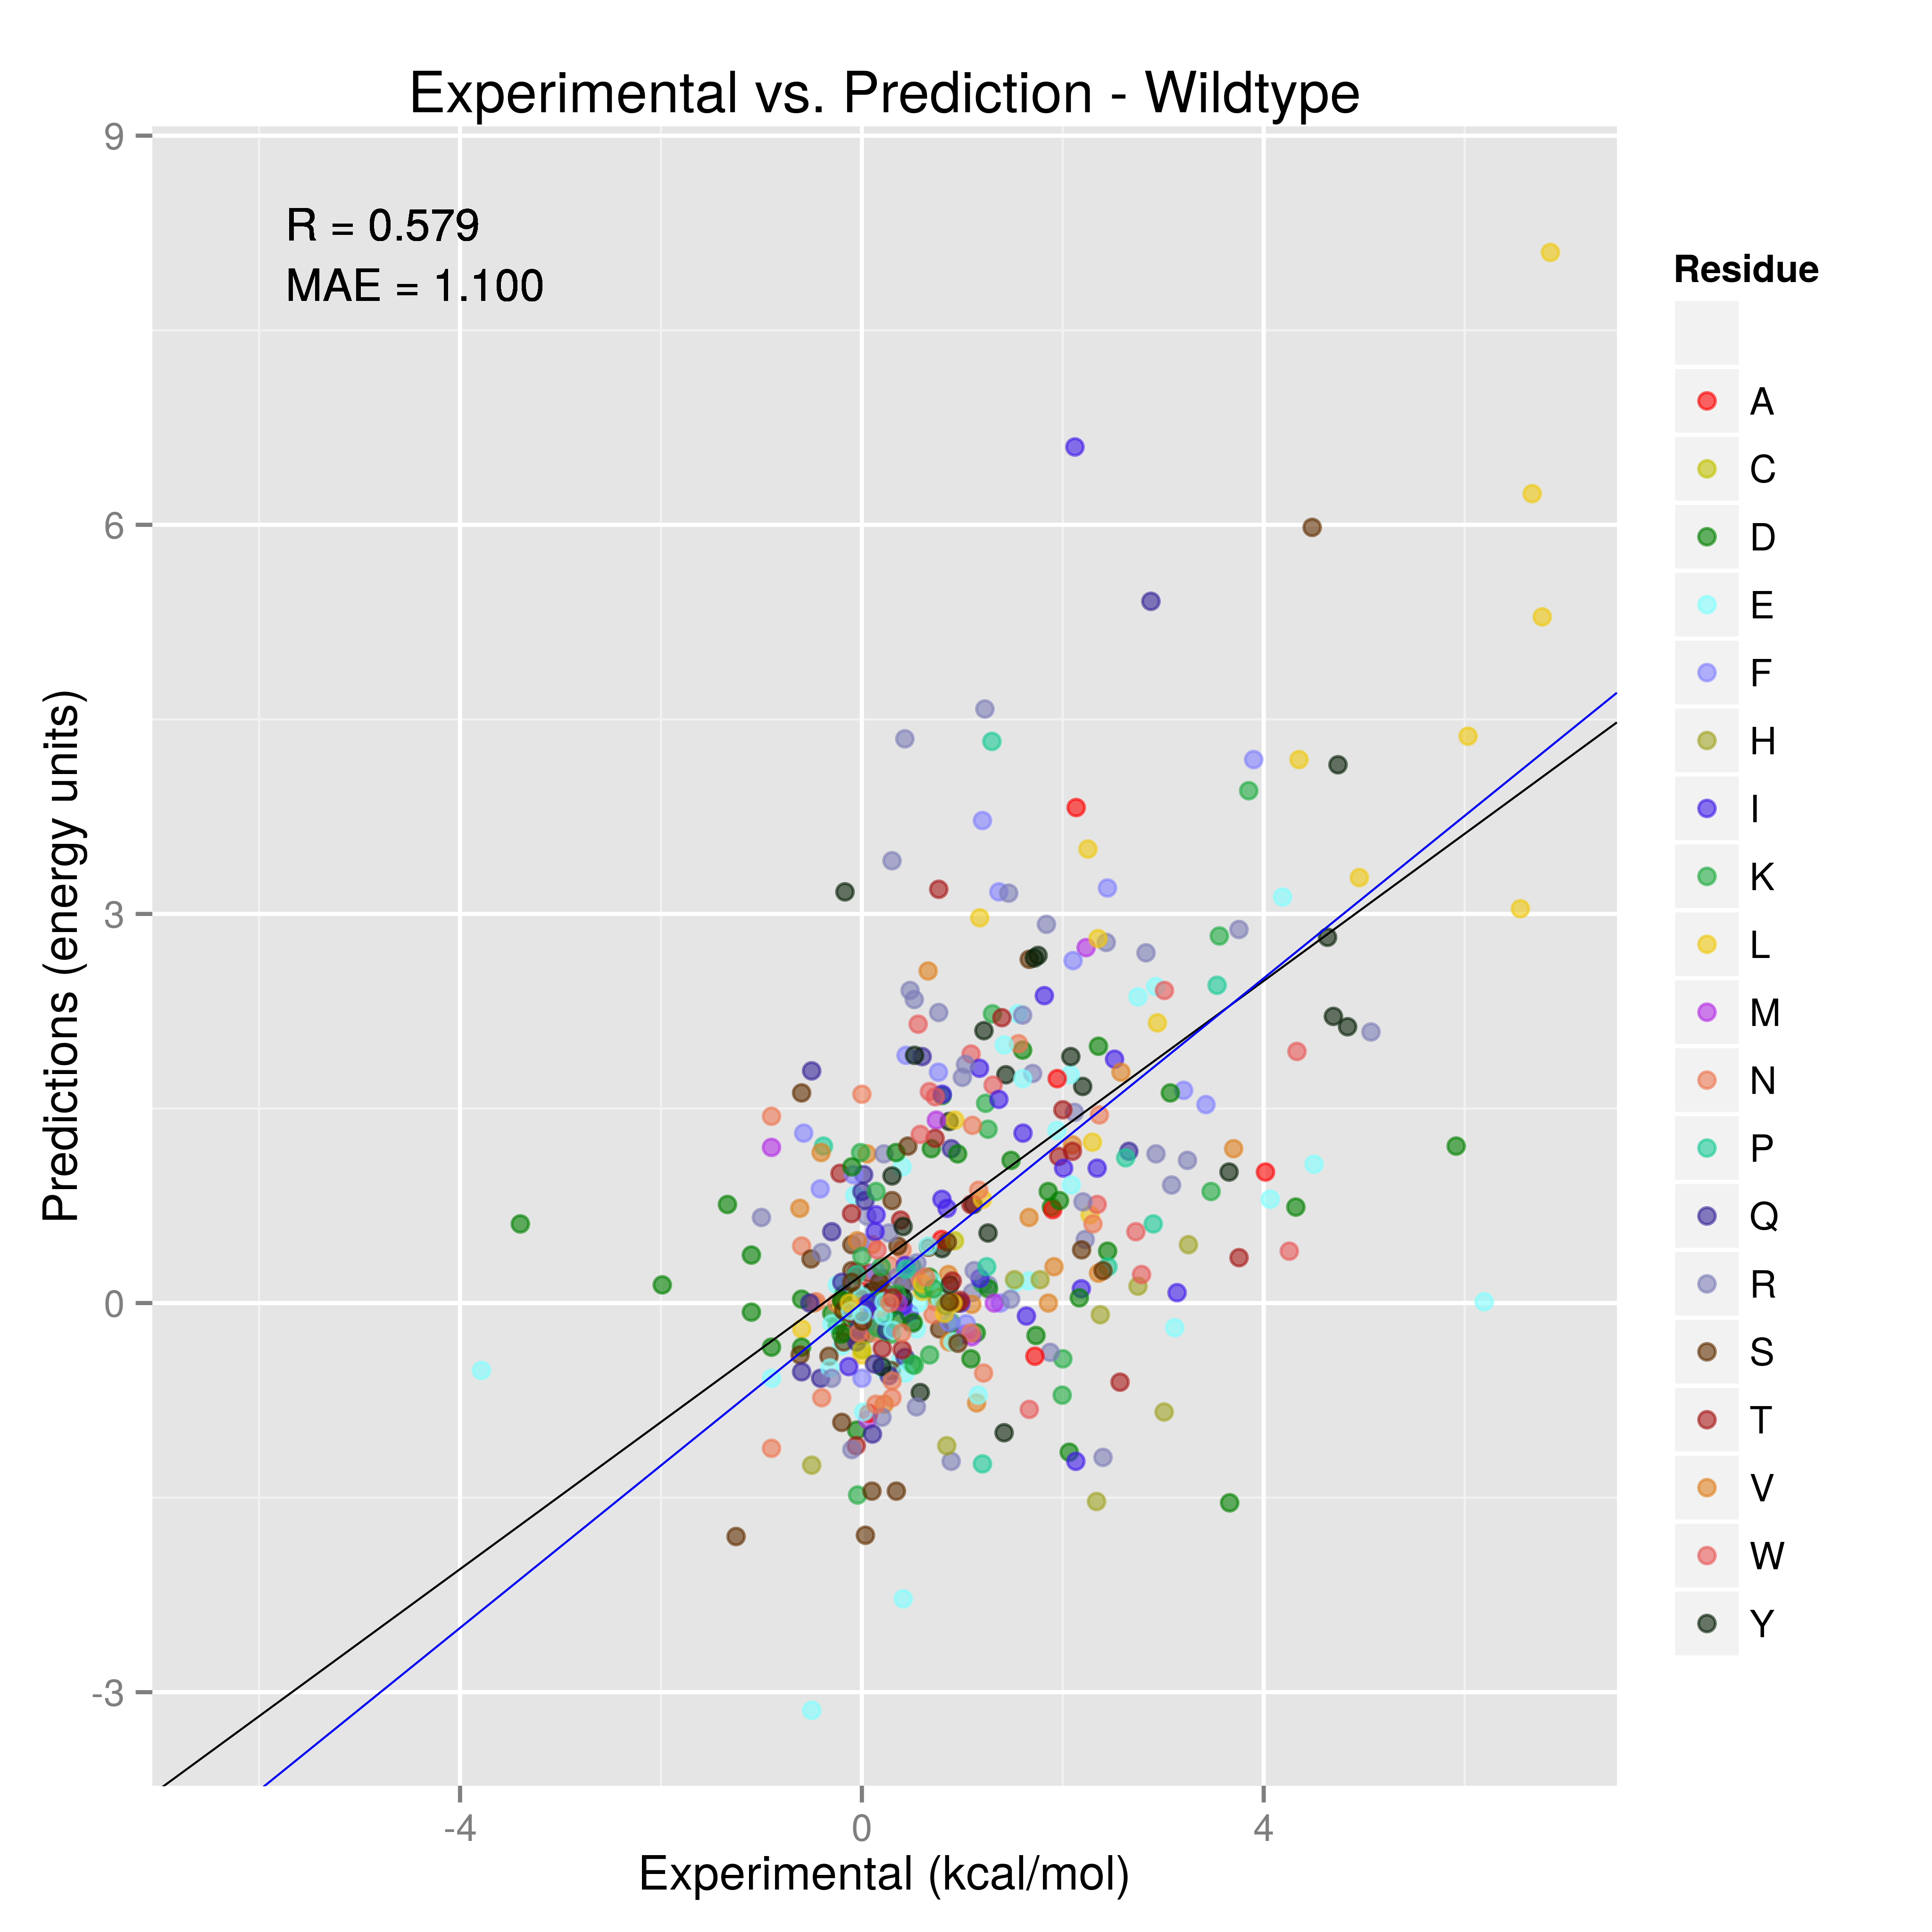
\includegraphics[width=\textwidth]{{/tmp/kyleb/multiple_analysis/analysis_sets/ZEMu/topx_1-prediction_set_id_zemu-values-score_method_zemu-paper/zemu-values_subplots/zemu-values_ZEMu_scatterplot_wildtype_aa}.png}
  \caption{Experimental vs. Prediction - Wildtype}
\end{figure}
\begin{figure}[H]
  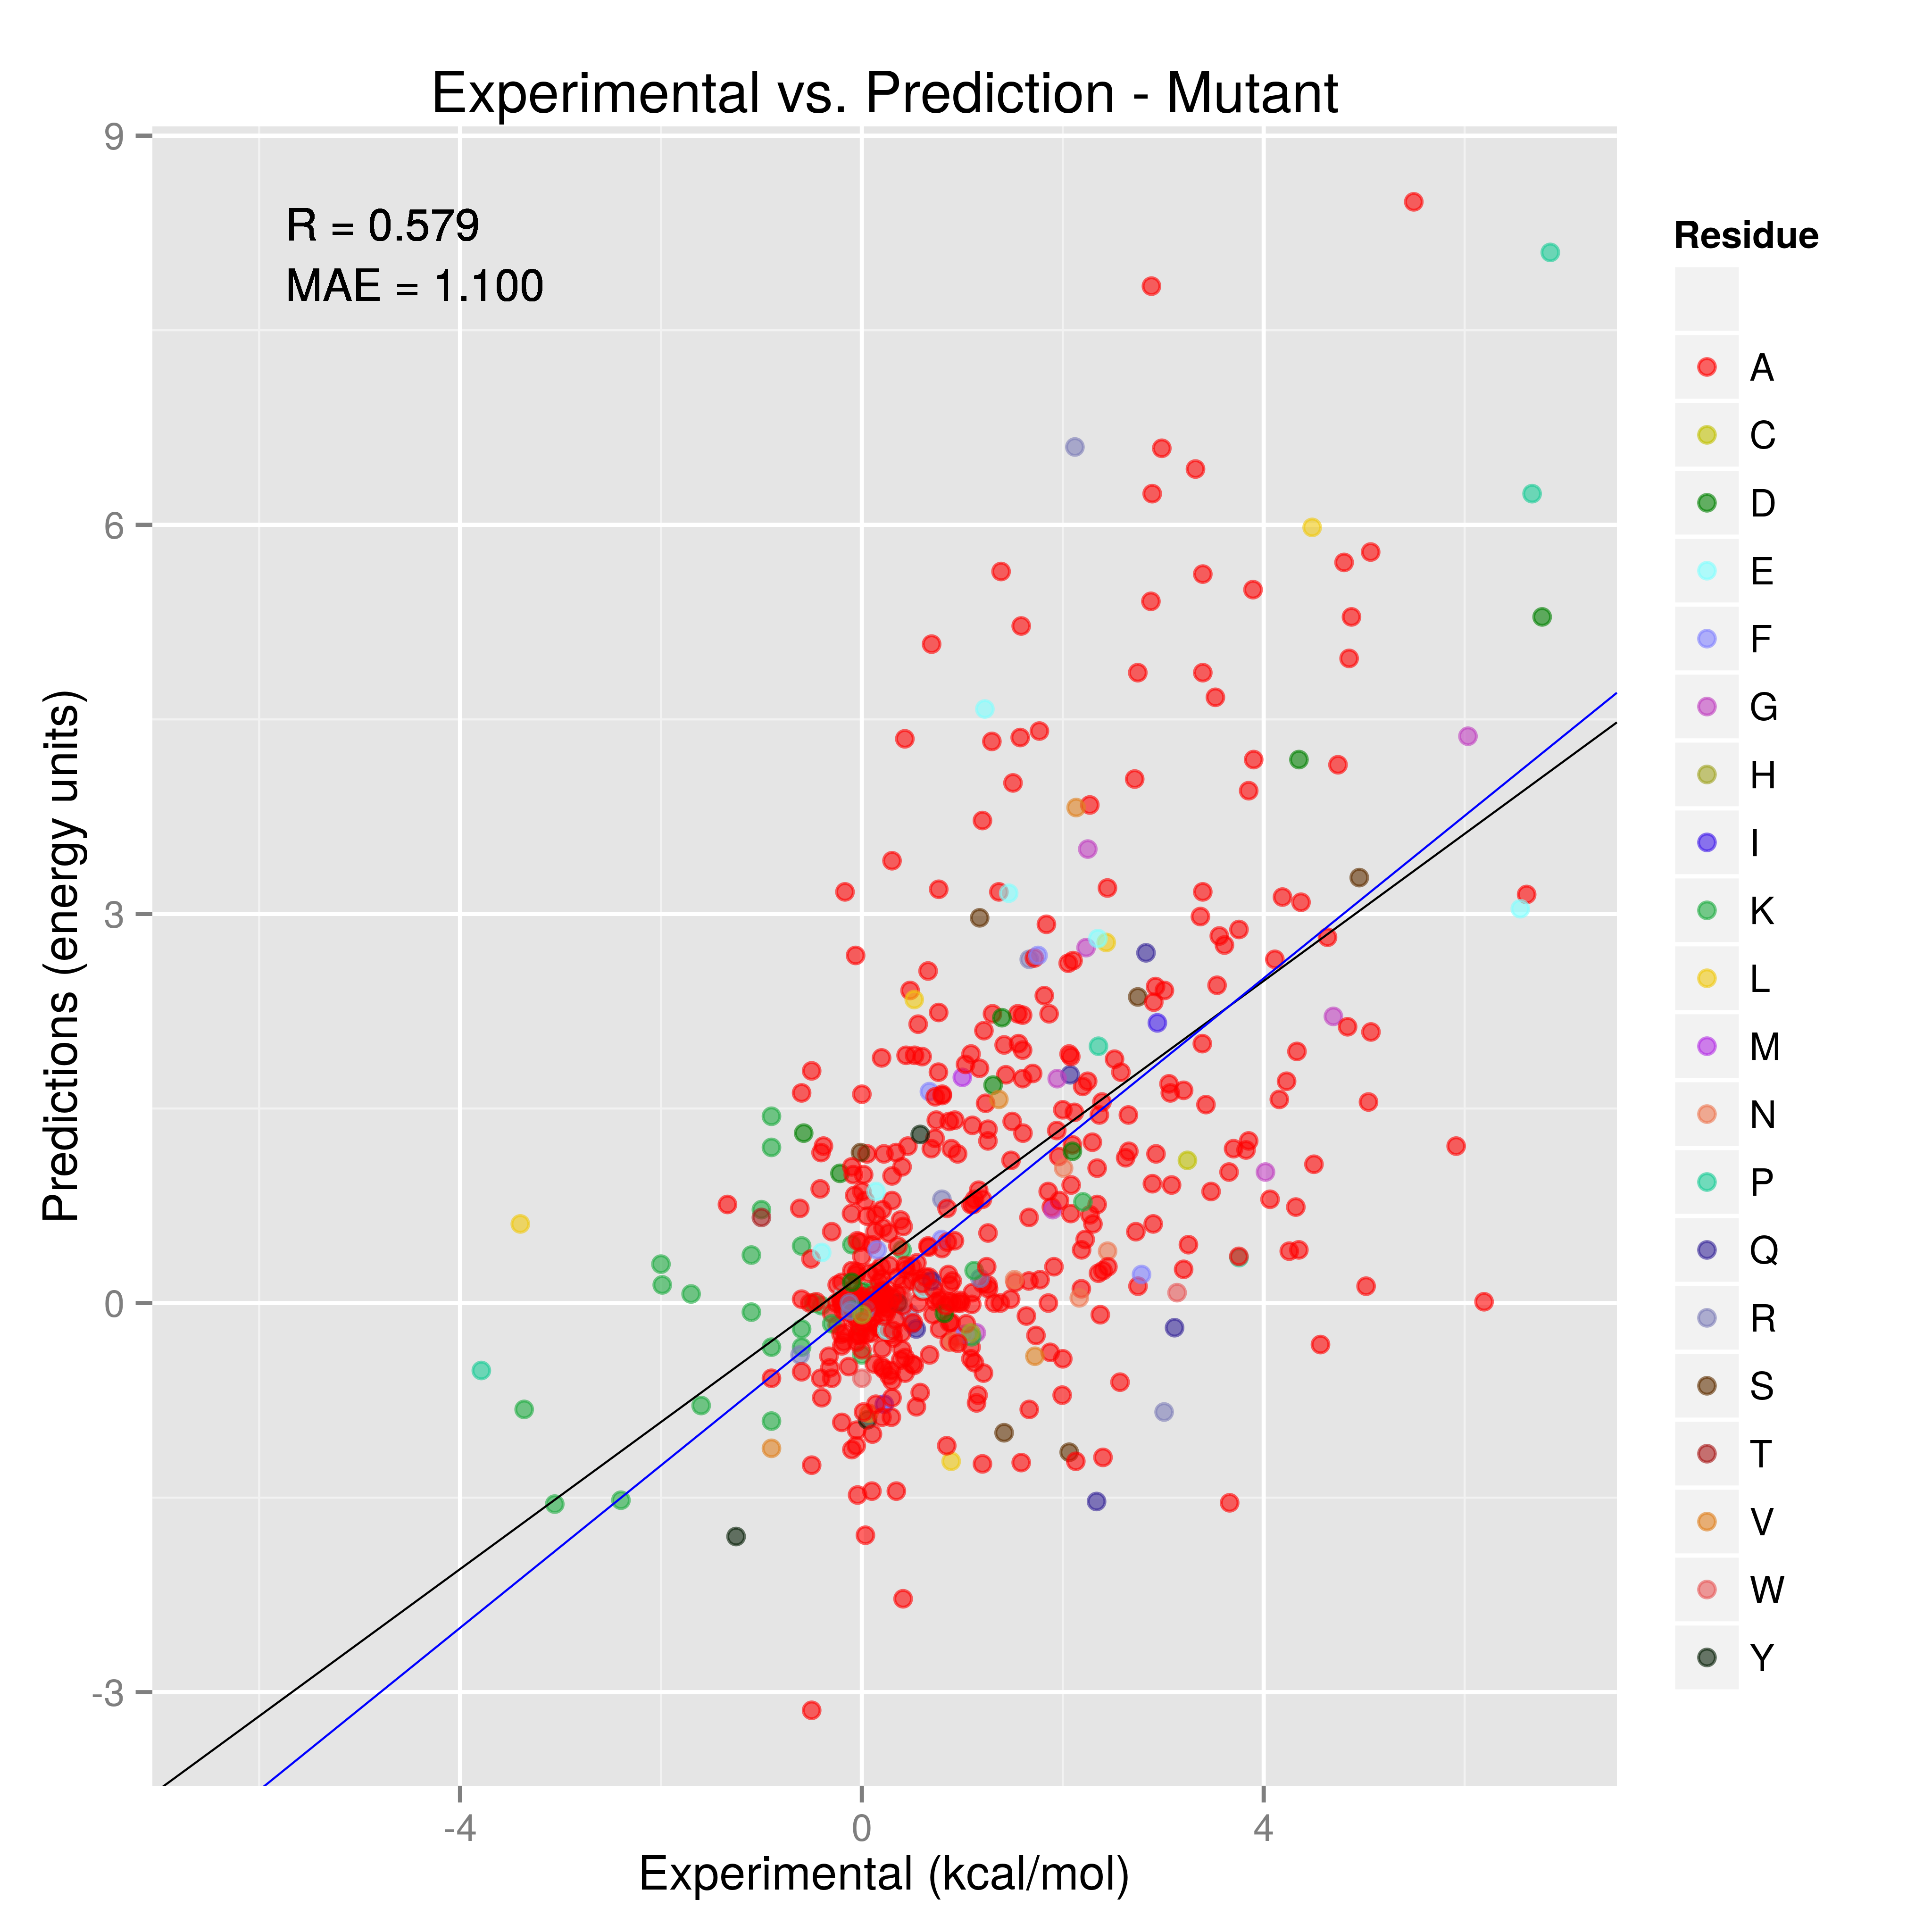
\includegraphics[width=\textwidth]{{/tmp/kyleb/multiple_analysis/analysis_sets/ZEMu/topx_1-prediction_set_id_zemu-values-score_method_zemu-paper/zemu-values_subplots/zemu-values_ZEMu_scatterplot_mutant_aa}.png}
  \caption{Experimental vs. Prediction - Mutant}
\end{figure}
\begin{figure}[H]
  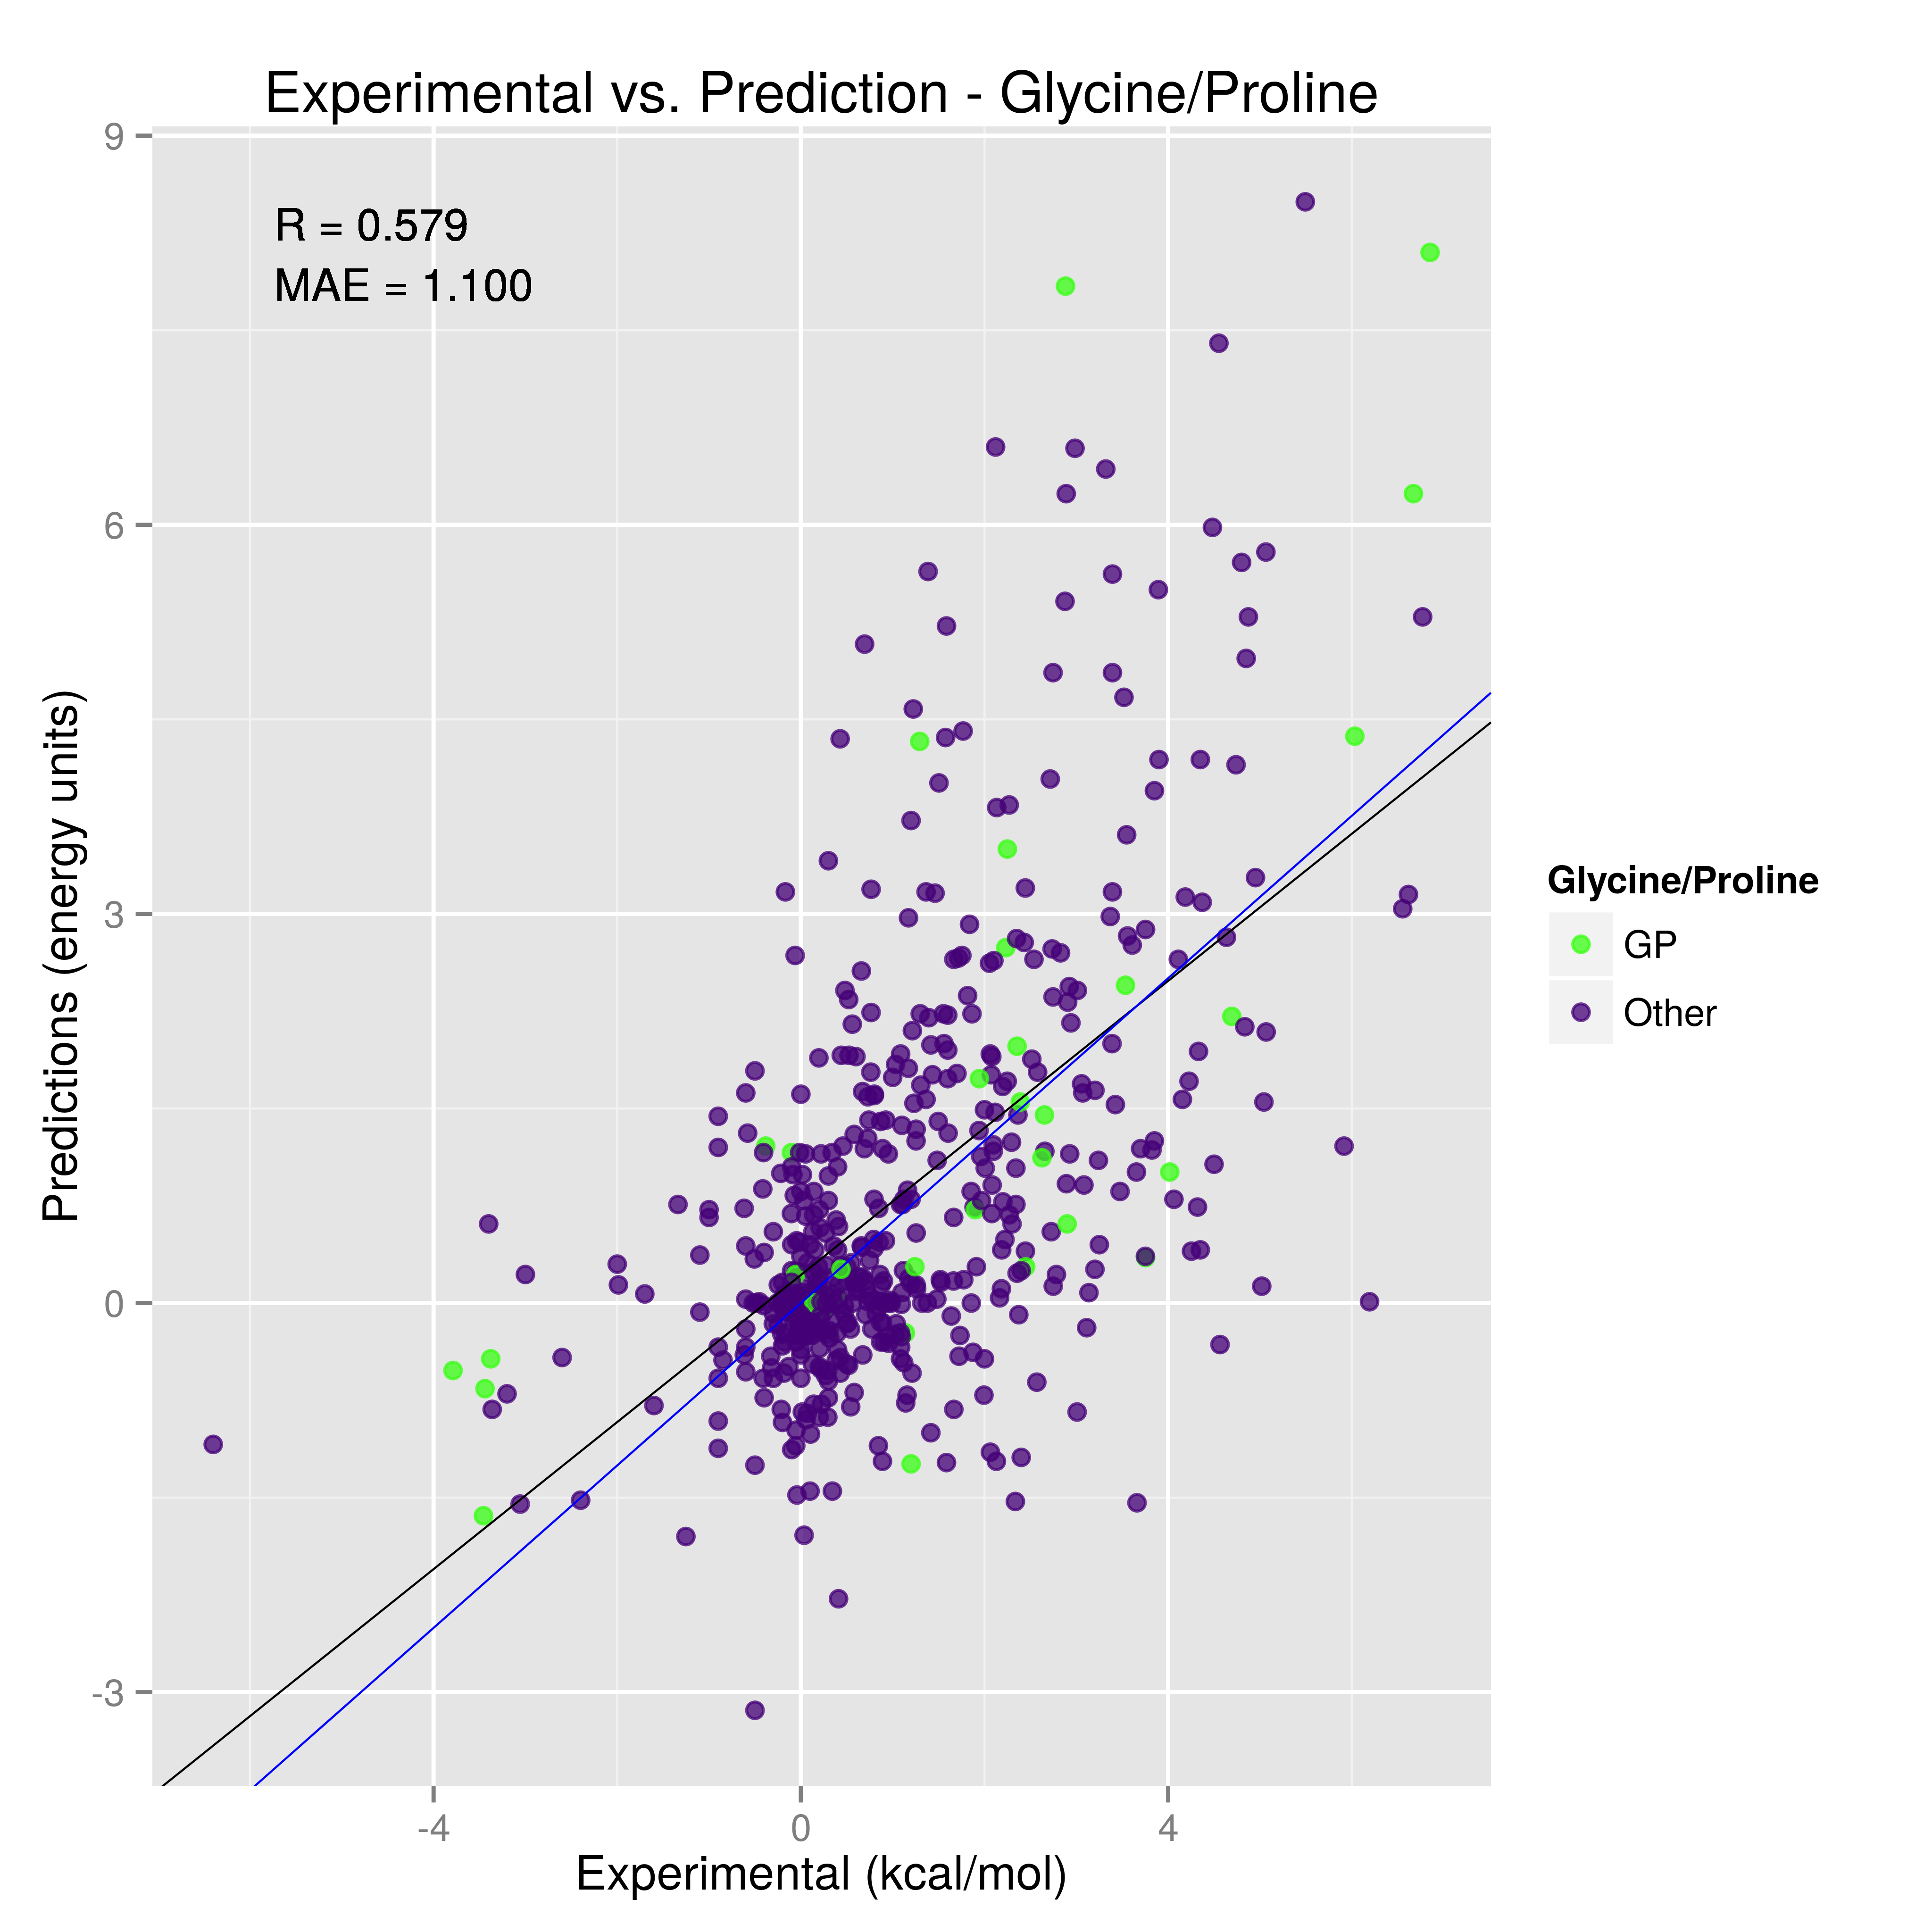
\includegraphics[width=\textwidth]{{/tmp/kyleb/multiple_analysis/analysis_sets/ZEMu/topx_1-prediction_set_id_zemu-values-score_method_zemu-paper/zemu-values_subplots/zemu-values_ZEMu_scatterplot_gp}.png}
  \caption{Experimental vs. Prediction - Glycine/Proline}
\end{figure}

\clearpage

\section{Chain properties}

\begin{figure}[H]
  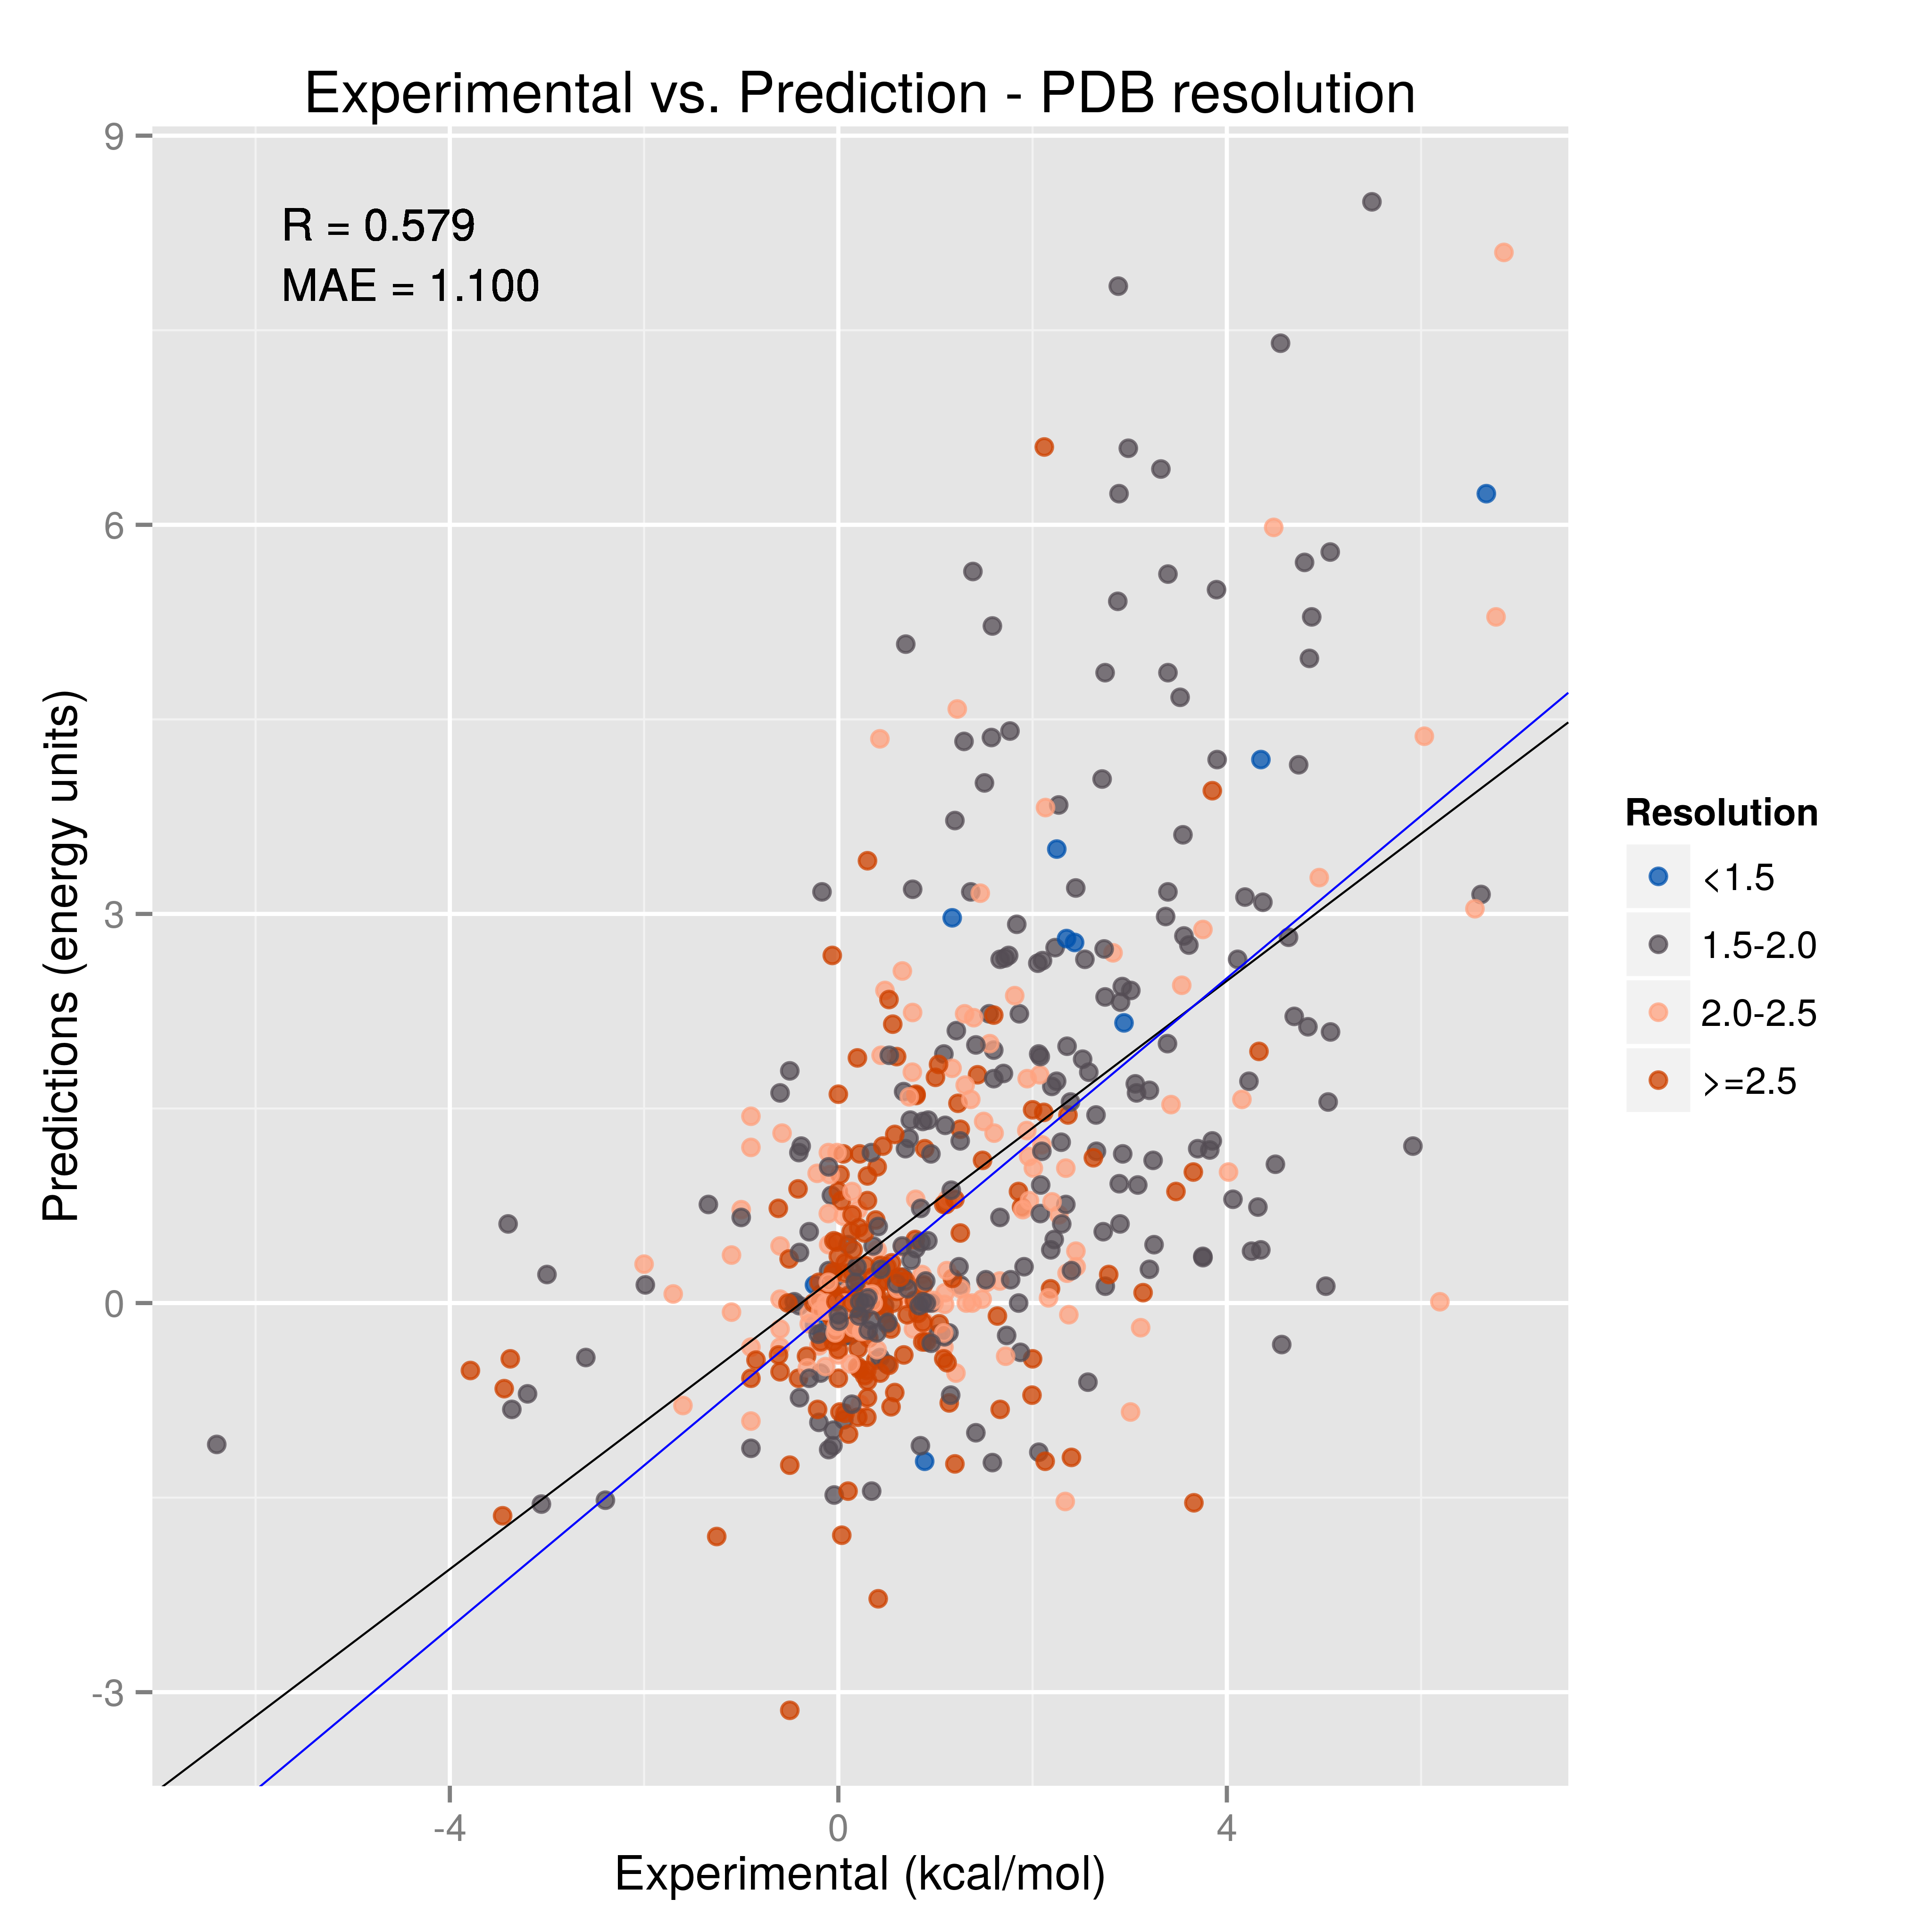
\includegraphics[width=\textwidth]{{/tmp/kyleb/multiple_analysis/analysis_sets/ZEMu/topx_1-prediction_set_id_zemu-values-score_method_zemu-paper/zemu-values_subplots/zemu-values_ZEMu_scatterplot_pdb_res_binned}.png}
  \caption{Experimental vs. Prediction - PDB resolution}
\end{figure}
\begin{figure}[H]
  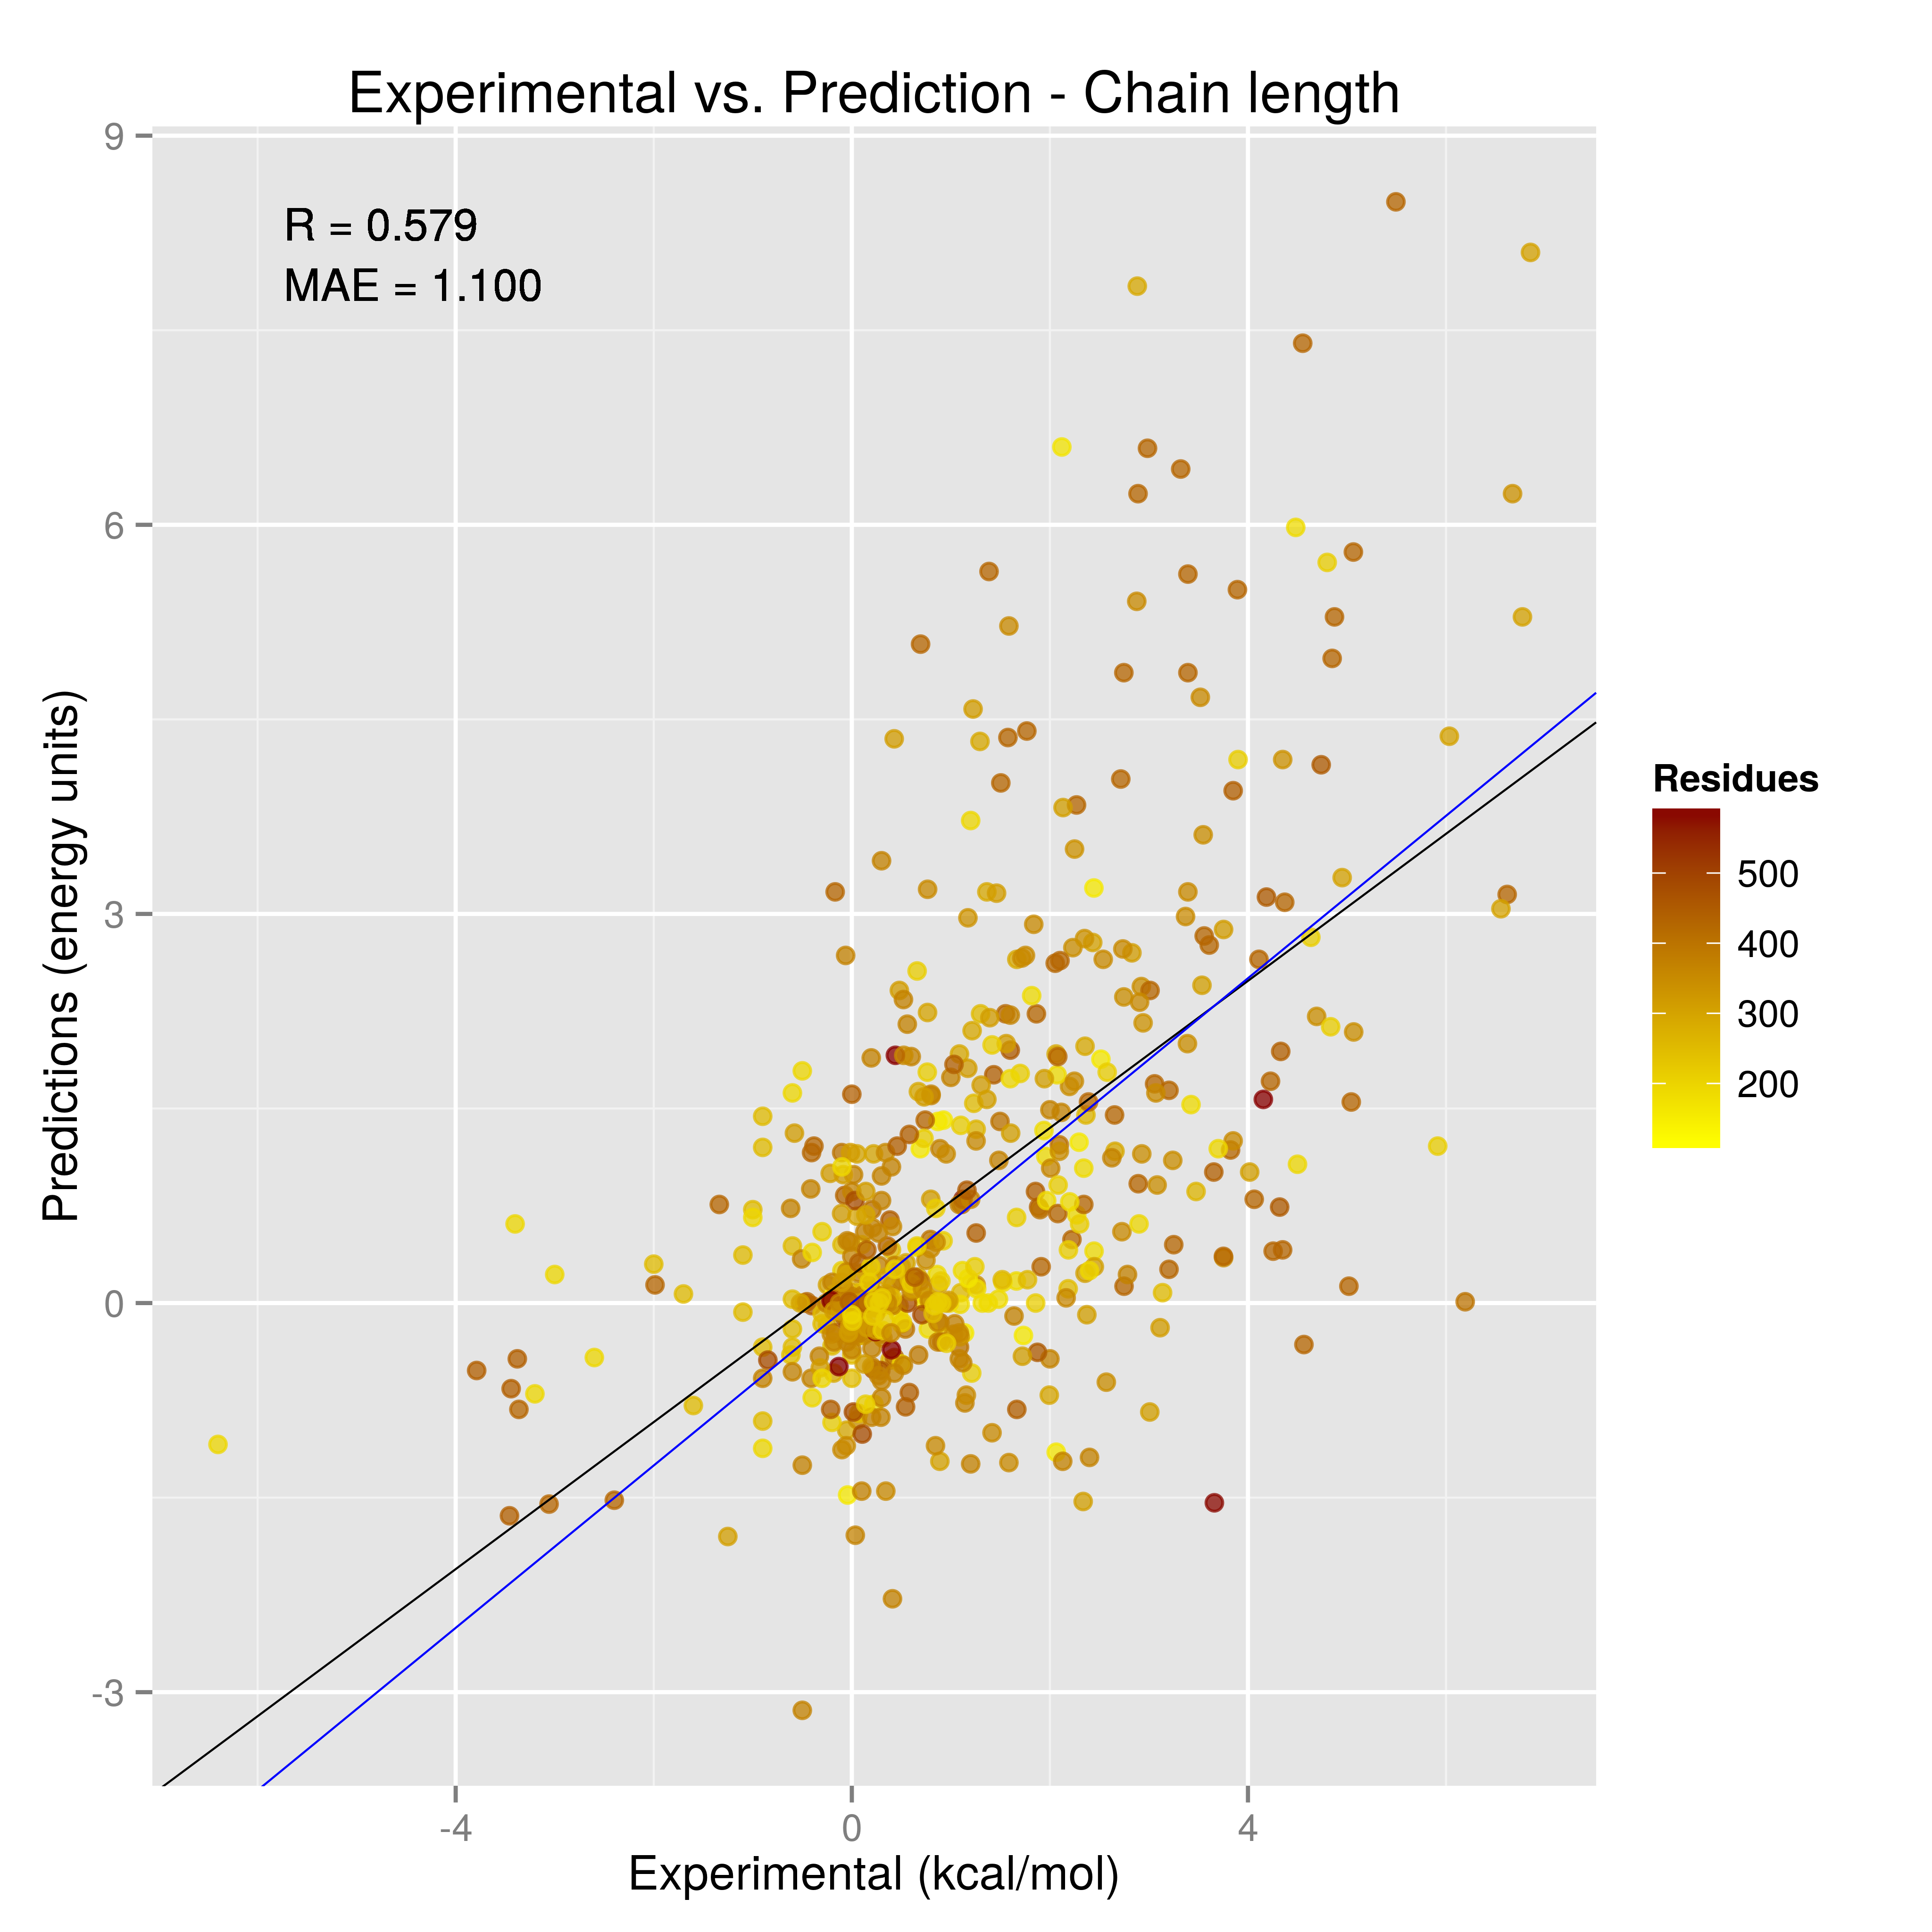
\includegraphics[width=\textwidth]{{/tmp/kyleb/multiple_analysis/analysis_sets/ZEMu/topx_1-prediction_set_id_zemu-values-score_method_zemu-paper/zemu-values_subplots/zemu-values_ZEMu_scatterplot_chain_length}.png}
  \caption{Experimental vs. Prediction - Chain length}
\end{figure}

\clearpage

\section{Errors / debugging}

\begin{figure}[H]
  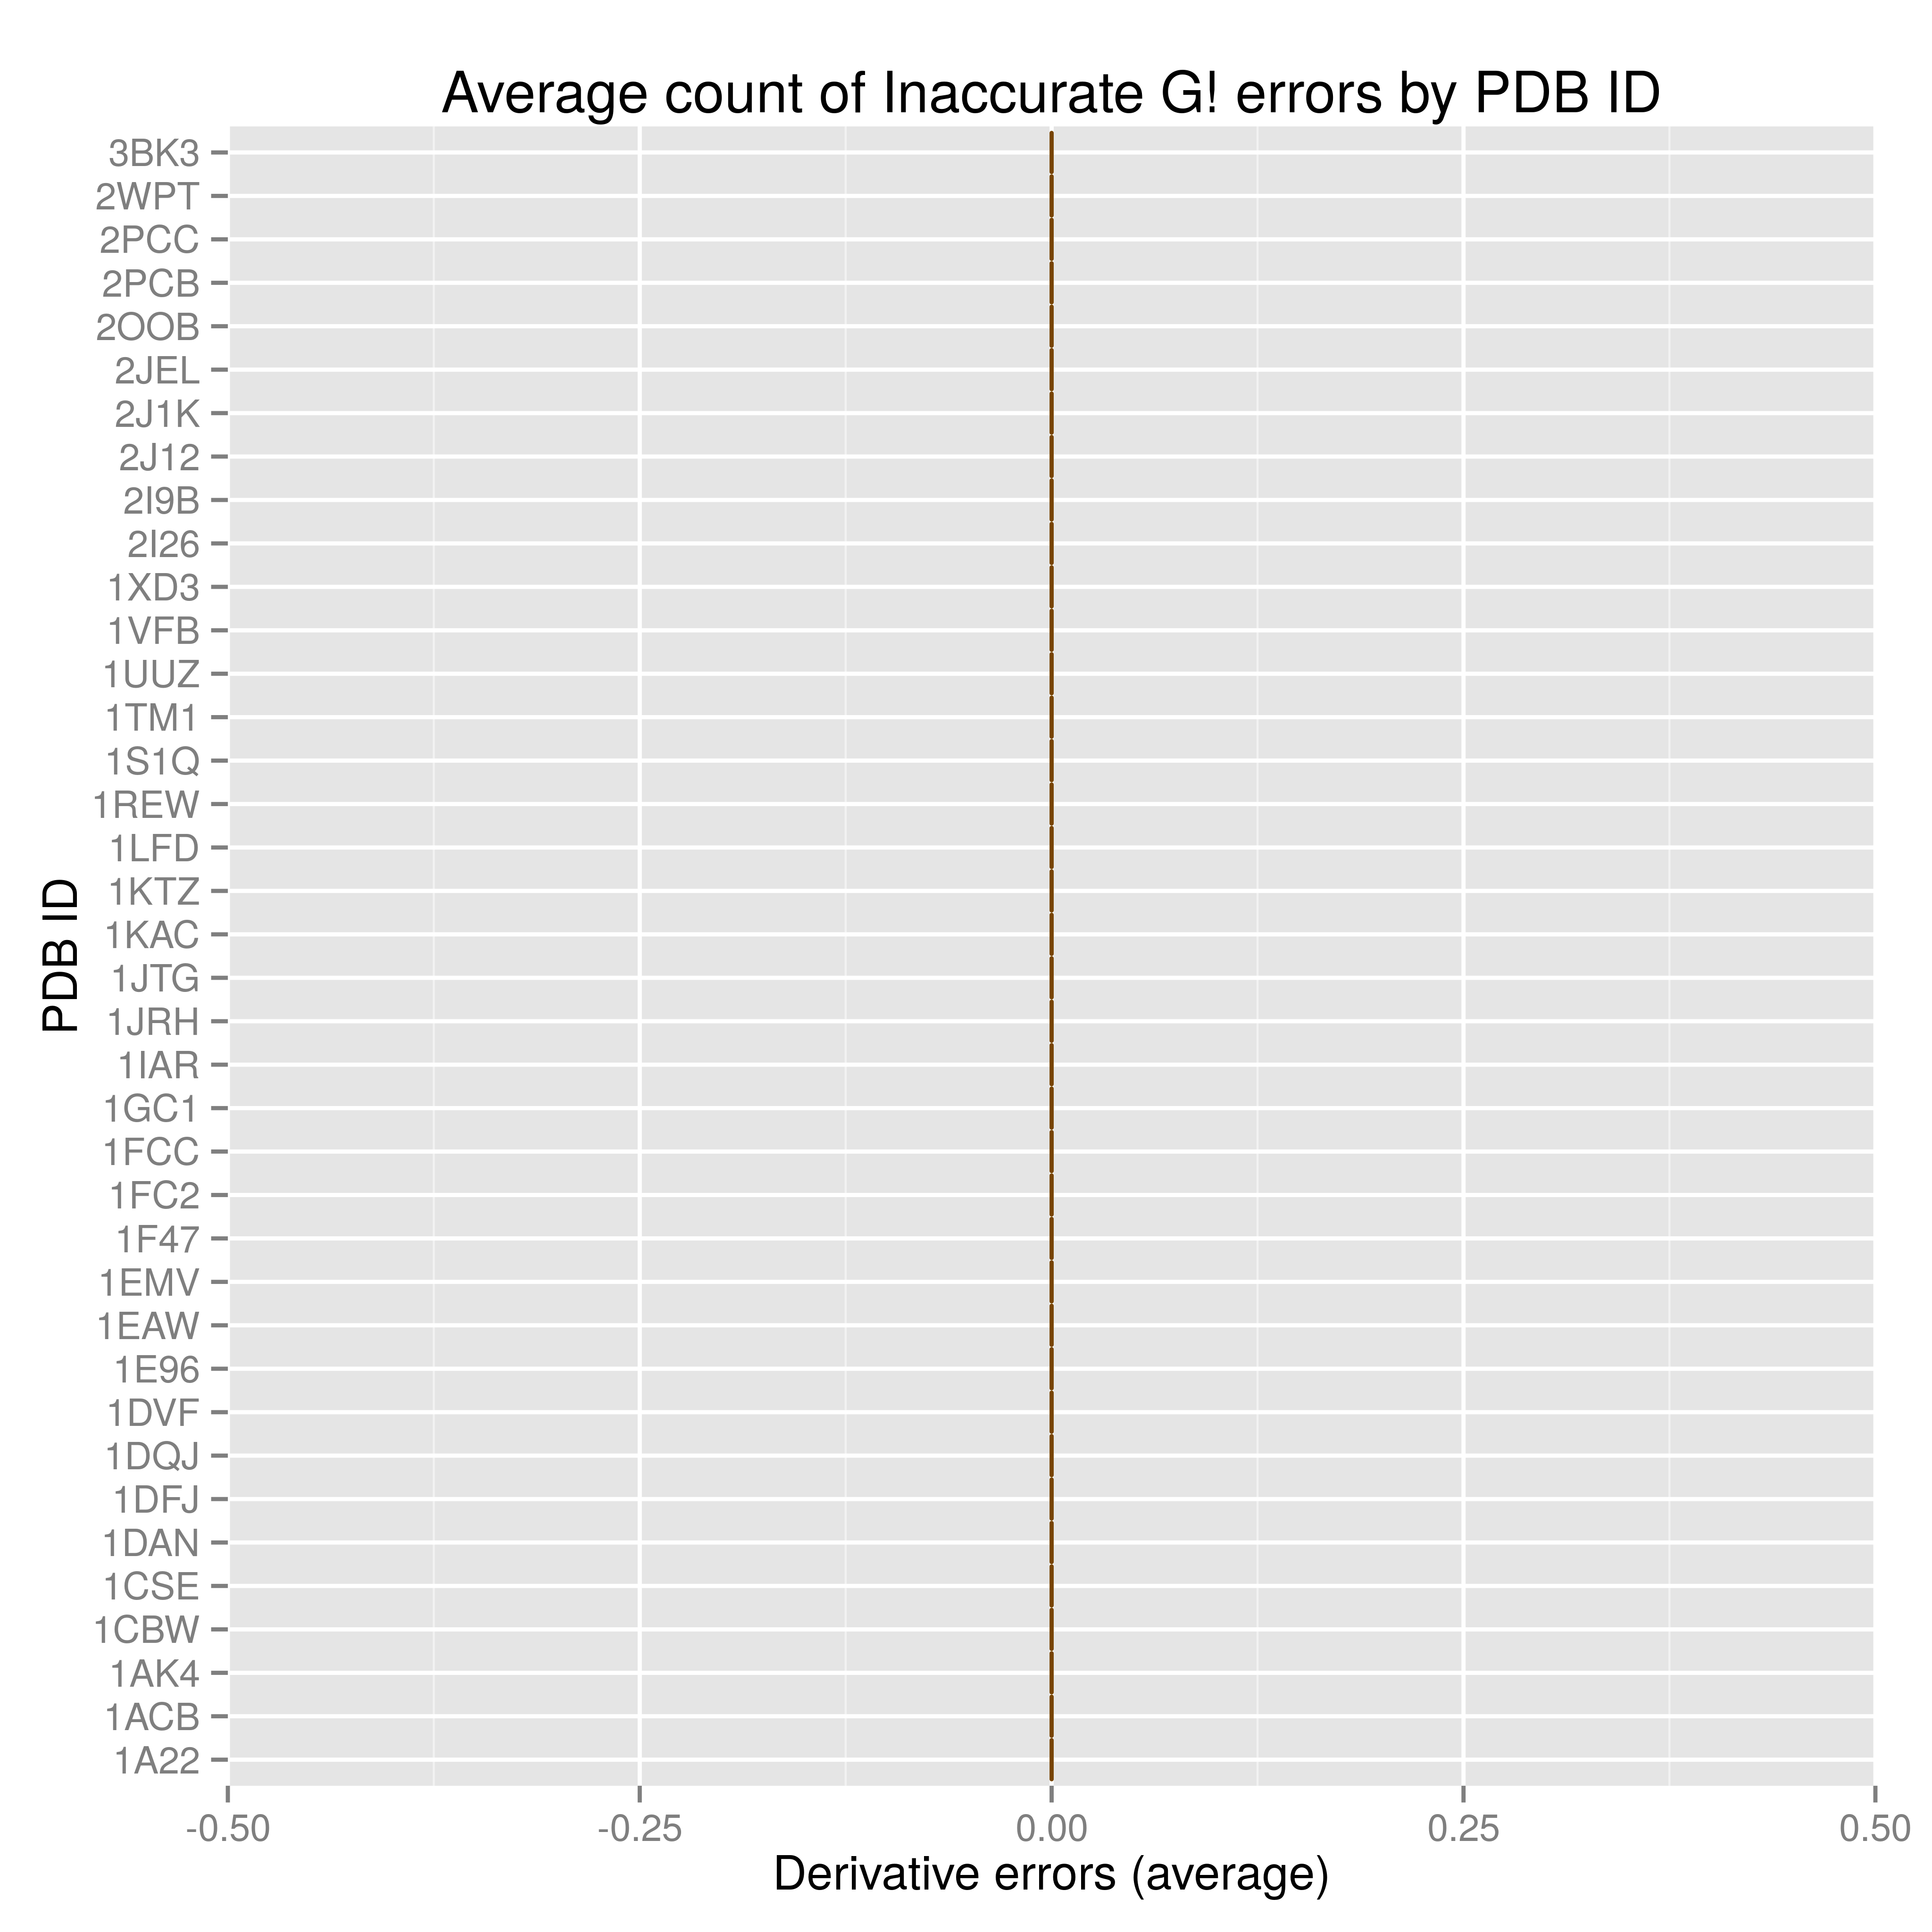
\includegraphics[width=\textwidth]{{/tmp/kyleb/multiple_analysis/analysis_sets/ZEMu/topx_1-prediction_set_id_zemu-values-score_method_zemu-paper/zemu-values_subplots/zemu-values_ZEMu_errors_by_pdb_id}.png}
  \caption{Derivative error barchart}
\end{figure}
\end{document}
